%% LaTeX Beamer presentation template (requires beamer package)
%% see http://bitbucket.org/rivanvx/beamer/wiki/Home
%% idea contributed by H. Turgut Uyar
%% template based on a template by Till Tantau
%% this template is still evolving - it might differ in future releases!

\documentclass[16pt]{beamer}

\mode<presentation>

\usetheme{Malmoe}
\useoutertheme{infolines}
\useinnertheme{default}
\setbeamercovered{transparent}
\setbeamertemplate{itemize items}[circle]  % itemize circles
\renewcommand\textbullet{\ensuremath{\bullet}}  % no error for bullets
\setbeamertemplate{caption}[numbered]      % numbered captions
\beamertemplatenavigationsymbolsempty

% PACKAGES + MODIFICATIONS

\usepackage[ngerman]{babel} %language and fonts
\usepackage[utf8]{inputenc}
\usepackage{lmodern}
\usepackage{textgreek}
\usepackage{textcomp} %for ° symbol


\usepackage{amsmath}	% math, use [fleqn] for equations on the left
\usepackage{amssymb}	% more symbols
%\usepackage{mathtools}  % for := (\coloneqq)

\usepackage{graphicx}	%graphics

\usepackage{feynmf}		% feynman graphs
\DeclareGraphicsRule{*}{mf}{*}{}

\usepackage{pifont}% http://ctan.org/pkg/pifont
\newcommand{\cmark}{\ding{51}}%
\newcommand{\xmark}{\ding{55}}%

\usepackage{enumerate}	% better way to config enumerates

\usepackage{tikz}		% flexible arrows
\usetikzlibrary{tikzmark,positioning}

\usepackage[skins,theorems]{tcolorbox}	%colored box
\tcbset{highlight math style={enhanced,colframe=red,colback=white,arc=0pt,boxrule=1pt}}

\usepackage{booktabs} % nicer hlines in tables

\usepackage{siunitx}
\sisetup{input-symbols = {()\%},  % do not treat "(", ")" and "%" in any special way
         group-digits  = false} % no grouping of digits

\usepackage{braket}
% NEW COMMANDS
\newcommand{\difd}{\mathrm{d}}							% differential d
\newcommand{\abs}[1]{\left|#1\right|}					% |.|
\newcommand{\avg}[1]{\left\langle#1\right\rangle}		% <.>
\newcommand{\dfour}{\delta^{(4)}}						% 4-dim. delta-distribution
\newcommand{\const}{const.}								% const.
\newcommand{\tptm}{{\tau^+ \tau^-}}						% \tau^+ \tau-
\newcommand{\qqbar}{\text{q} \bar{\text{q}}}			% q q~
\newcommand{\mathematica}{\textsc{Mathematica}}			% Mathematica in small capitals
\newcommand{\mg}{\textsc{MadGraph}}						% MadGraph in small capitals
\newcommand{\mgfive}{\textsc{MadGraph}~5}				% MadGraph in small capitals with version number
\newcommand{\vegas}{VEGAS}								% VEGAS
\newcommand{\cuba}{\textsc{Cuba}}						% Cuba in small capitals
\newcommand{\unit}[1]{\,\text{#1}}						% physical unit
\newcommand{\matrixm}{\mathcal{M}}						% matrix element M
\newcommand<>{\uncoverubrace}[2]{
  \onslide#3 \underbrace{ \onslide<1->
  #1
  \onslide#3 }_{#2} \onslide<1->
}
\newcommand{\emptynl}{\mbox{}\\}						% empty new line
\newcommand\textbox[1]{									% textbox for hor. alignment
	\parbox{.333\textwidth}{#1}%
}

\DeclareMathOperator{\sgn}{sgn}

% DOCUMENT SETTINGS

\title{$Z^0$ Resonanz am LEP}
\subtitle{FP II Präsentation}
\author{B. Winkelmann, P. Spalthoff}
\institute{}
\date{27.04.2016}


% This is only inserted into the PDF information catalog. Can be left out.
\subject{\texorpdfstring{$Z^0$}{Z0} resonance at the LEP}

\begin{document}

\begin{frame}[noframenumbering, plain]
\titlepage
\end{frame}

\begin{frame}[noframenumbering]
\frametitle{Inhalt}
\tableofcontents[hideallsubsections]
\end{frame}

\AtBeginSection[]
{
\begin{frame}<beamer>[noframenumbering]
\frametitle{}
\tableofcontents[currentsection,hideothersubsections]
\end{frame}
}

% \begin{frame}
% 	\frametitle{Wirkungsquerschnitt}
% 	\begin{figure}
% 	\begin{center}
% 	  \includegraphics[width=0.3\textwidth]{../img/atlas_higgs_event.png}
% 	  \caption{Produkte einer Proton-Proton-Kollision beim ATLAS-Experiment am CERN (Quelle: https://cds.cern.ch/record/1459496)}
% 	\end{center}
% 	\end{figure}
% 	\begin{itemize}
% 		\item Bei Streuprozessen ist der Endzustand nicht eindeutig bestimmt
% 		\item Der Wahrscheinlichkeit eines bestimmten Endzustandes wird durch den Wirkungsquerschnitt $\sigma$ beschrieben.
% 		\item Differentieller Wirkungsquerschnitt $\frac{\difd \sigma}{\difd O}$ in Bezug auf \\
% 			  Observable $O$ (z.B. Raumwinkel $\Omega$, Transversalimpuls $p_\text{T}, \ldots$)
% 	\end{itemize}
% \end{frame}

\section{Theoretische Grundlagen}

\subsection{Das Standardmodell}
 \begin{frame}
 	\frametitle{Das Standardmodell}
 	\begin{figure}
 	\begin{center}
 	  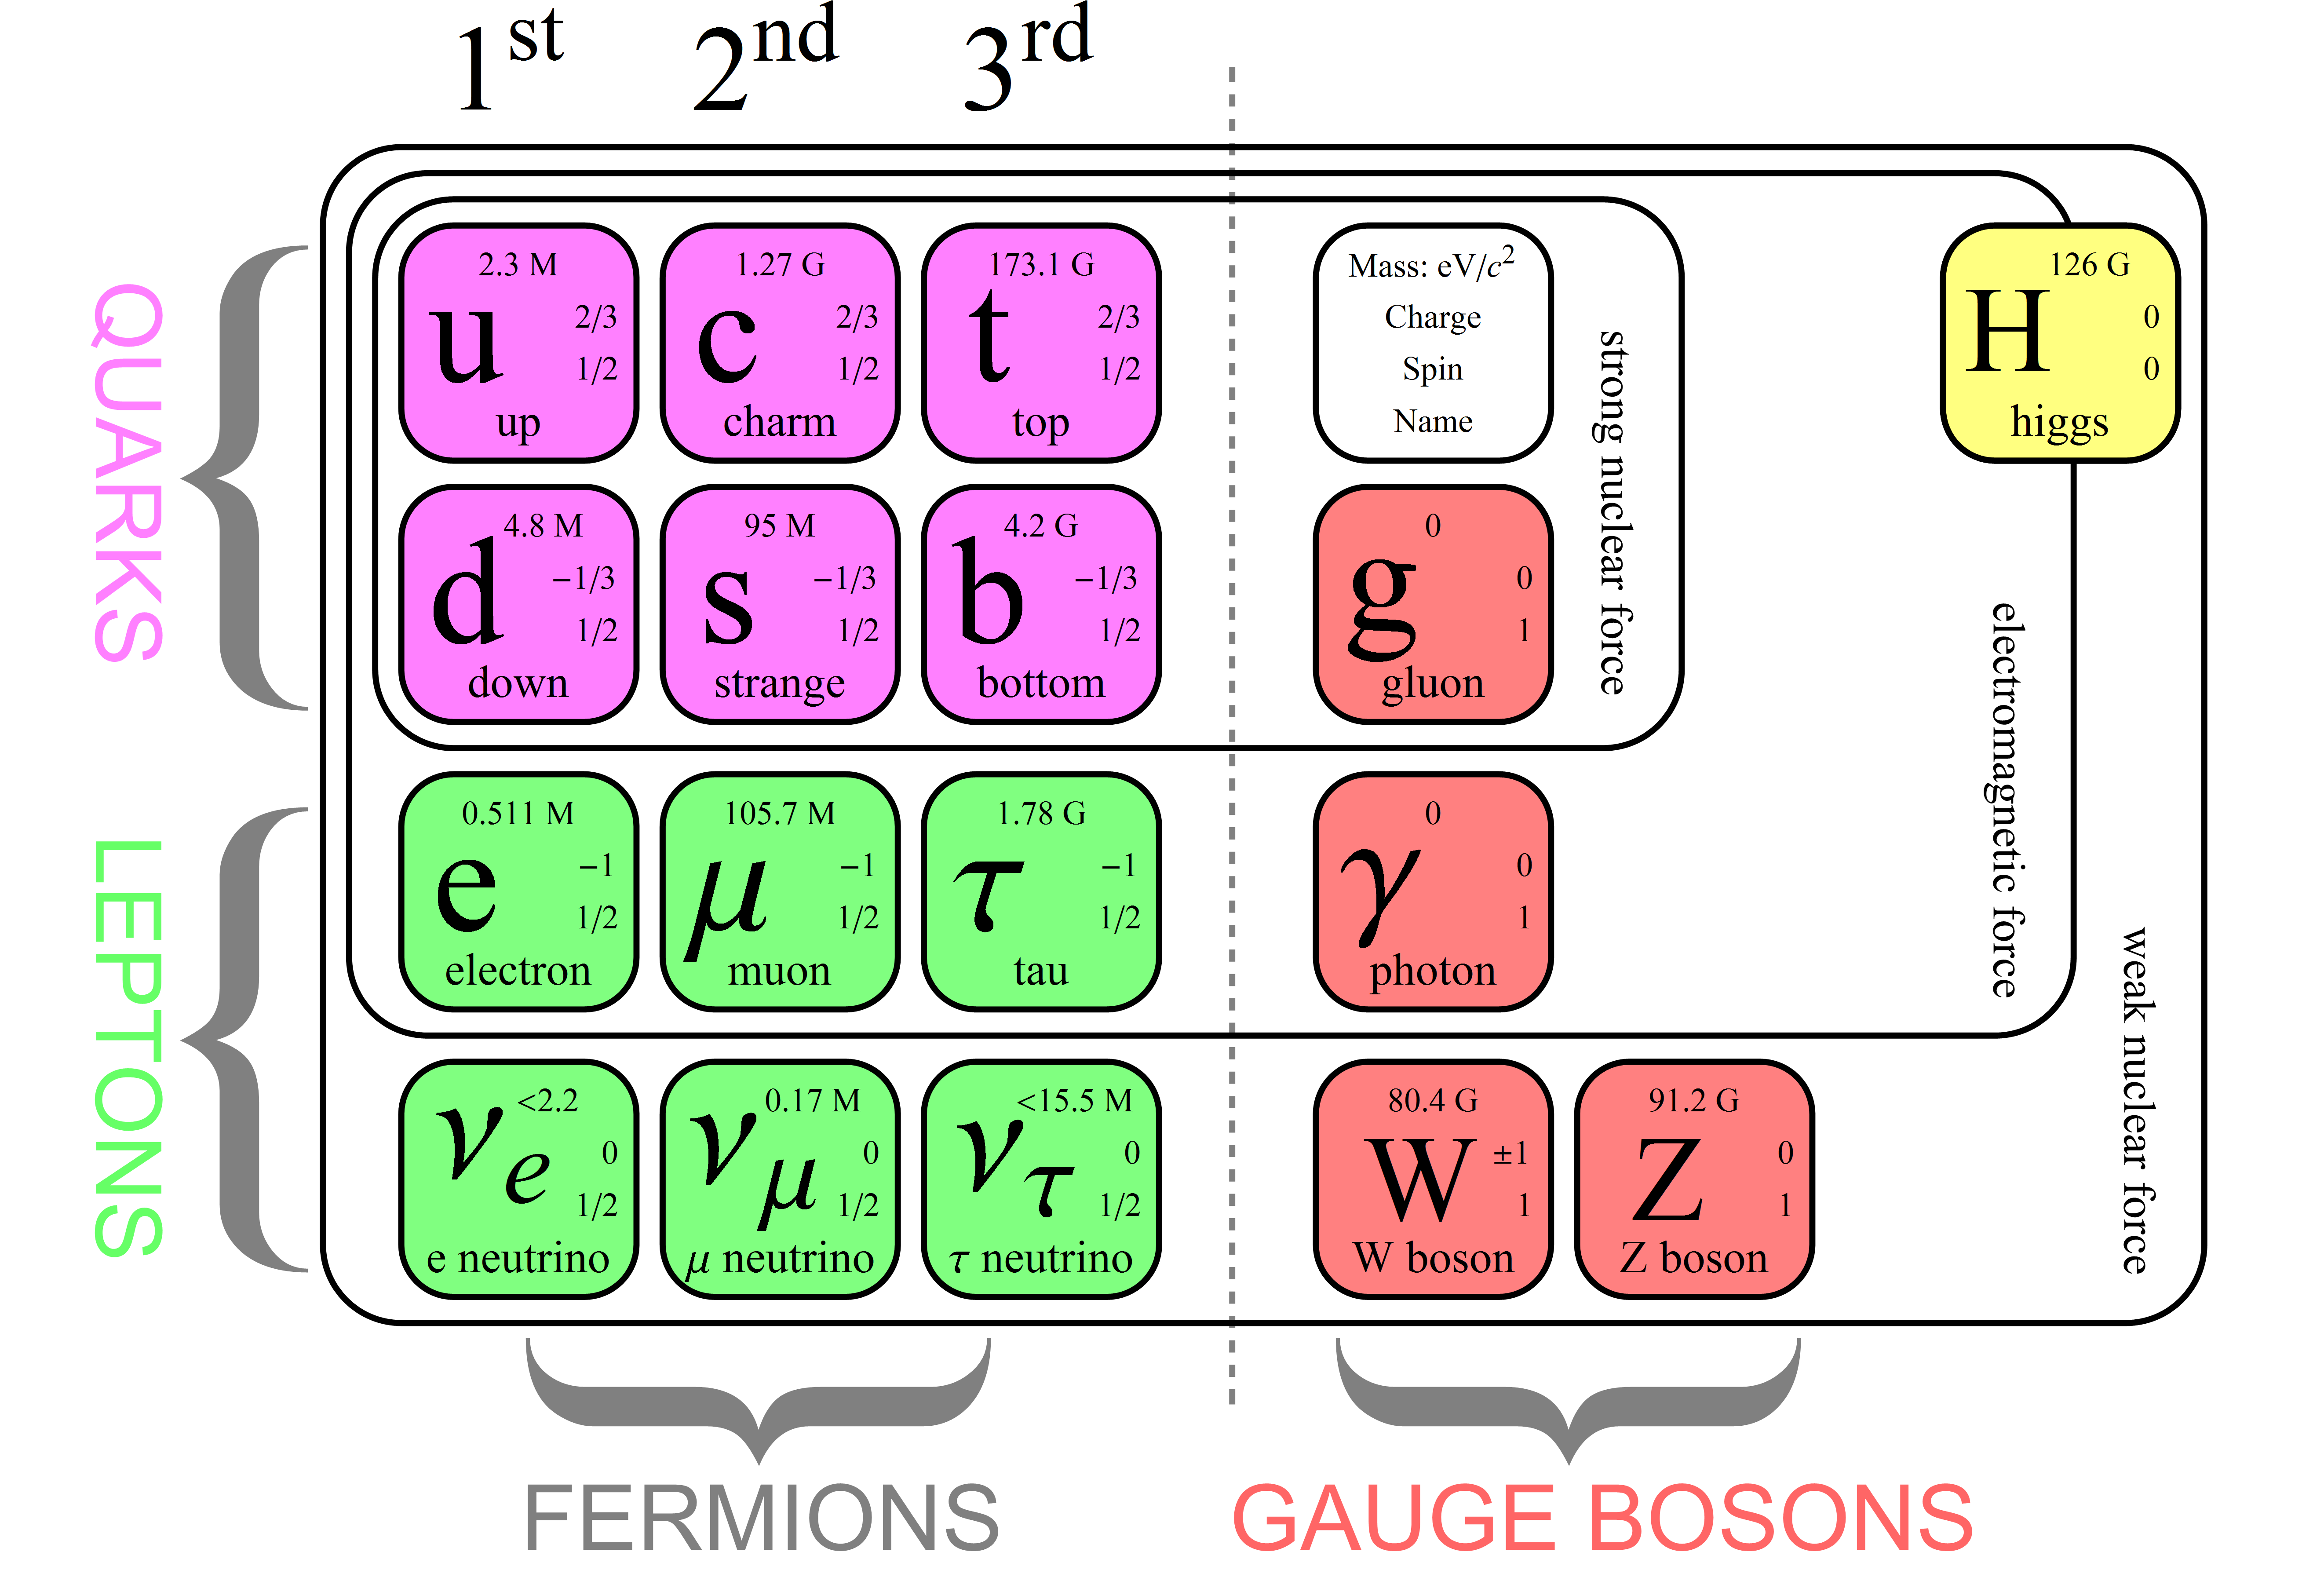
\includegraphics[width=0.9\textwidth]{graphics/SM1.png}
 	\end{center}
	\end{figure}
 \end{frame}
\subsection{Elektroschwache Wechselwirkung}
\begin{frame}
	\frametitle{Weinbergwinkel und Kopplungsstärken}
	\begin{center}
		\begin{equation*}
			\ket{\gamma} =  cos(\theta_w)\ket{B^0} + sin(\theta_w) \ket{W^0}
		\end{equation*}
		\begin{equation*}
		\ket{Z^0} = -sin(\theta_w) \ket{B^0} + cos(\theta_w) \ket{W^0}
		\end{equation*}\\
		\begin{equation*}
		\textcolor{lightgray}{g_V^f = I^f_3-2 Q_f sin^2(\theta_w)}
		\end{equation*}
		\begin{equation*}
		\textcolor{lightgray}{g_A^f = I^f_3}
		\end{equation*}
	\end{center}
\end{frame}
\begin{frame}
	\frametitle{Weinbergwinkel und Kopplungsstärken}
	\begin{center}
		\begin{equation*}
		\textcolor{lightgray}{\ket{\gamma} =  cos(\theta_w)\ket{B^0} + sin(\theta_w) \ket{W^0}}
		\end{equation*}
		\begin{equation*}
		\textcolor{lightgray}{\ket{Z^0} = -sin(\theta_w) \ket{B^0} + cos(\theta_w) \ket{W^0}}
		\end{equation*}
		\\
		\begin{equation*}
			g_V^f = I^f_3-2 Q_f sin^2(\theta_w)
		\end{equation*}
		\begin{equation*}
			g_A^f = I^f_3
		\end{equation*}
	\end{center}
\end{frame}

\subsection{$e^+e^-$ Kollisionen}
\begin{frame}
	\frametitle{$e^+e^- \rightarrow f\bar{f}$ }
	\begin{center}
		\begin{figure}
			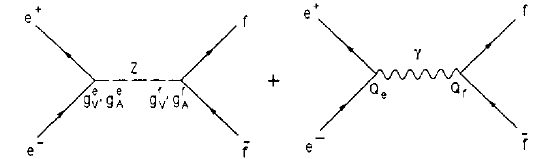
\includegraphics[width=0.8\textwidth]{graphics/annihilation.png}
		\end{figure}
	\end{center}
\end{frame}
\begin{frame}
	\frametitle{Der Wirkungsquerschnitt}
	\begin{equation*}
		\sigma(s) = \frac{12\pi}{ \tikzmark{MZ1}M_Z^2}
		\frac{s\tikzmark{gammae}\Gamma_e \tikzmark{gammaf}\Gamma_f}{(s-\tikzmark{MZ2}M_Z^2)^2 + s^2\cdot\tikzmark{gammaZ}\Gamma_Z^2 / \tikzmark{MZ3}M_Z^2}
	\end{equation*}
	\begin{tikzpicture}[
	remember picture,
	overlay,
	expl1/.style={draw=orange,fill=orange!30,rounded corners},
	expl2/.style={draw=gray!20,fill=gray!10,rounded corners},
	arrow1/.style={red!80!black,ultra thick,->,>=latex},
	arrow2/.style={gray!20,ultra thick,->,>=latex}
	]
	\node[expl1]
	(gammaeexpl)
	at (2,2cm)
	{\textcolor{black}{Zerfallsbreite Elektron}};
	\node[expl1]
	(gammafexpl)
	at (10,2cm)
	{\textcolor{black}{Zerfallsbreite Fermion}};
	\node[expl1]
	(MZexpl)
	at (1,-1cm)
	{Masse $Z^0$};
	\node[expl1]
	(gammaZexpl)
	at (9.8,-1cm)
	{\textcolor{black}{Gesamtzerfallsbreite $Z^0$}};
	\draw[arrow1]
	(gammafexpl.west) to[out=180,in=90] ([yshift=-8.2ex,xshift=1.5ex]{pic cs:gammaf});
	\draw[arrow1]
	(gammaeexpl.east) to[out=0,in=90] ([yshift=2ex,xshift=0.5ex]{pic cs:gammae});
	\draw[arrow1]
	(gammaZexpl.west) to[out=180,in=270] ([yshift=-10.5ex,xshift=0.5ex]{pic cs:gammaZ});
	\draw[arrow1]
	(MZexpl.east) to[out=0,in=270] ([yshift=-10.5ex,xshift=1ex]{pic cs:MZ1});
	%\draw[arrow1]
	%(MZexpl.east) to[out=0,in=270] ([yshift=-10.5ex,xshift=1ex]{pic cs:MZ2});
	%\draw[arrow1]
	%(MZexpl.east) to[out=0,in=270] ([yshift=-10.5ex,xshift=1ex]{pic cs:MZ3});
	\end{tikzpicture}
\end{frame}
\begin{frame}
	\frametitle{Bhabha Streuung }
	\begin{center}
		\begin{figure}
			\includegraphics[width=0.8\textwidth]{graphics/Bhabbastreuung.png}
		\end{figure}
	\end{center}
	\begin{equation*}
	\frac{d\sigma_s}{d\Omega} \propto (1+cos^2(\theta)),\qquad\frac{d\sigma_t}{d\Omega}t \propto (1-cos(\theta))^{-2}
	\end{equation*}
\end{frame}
\subsection{Strahlungskorrekturen}
\begin{frame}
	\frametitle{Strahlungskorrekturen}
	\begin{figure}
		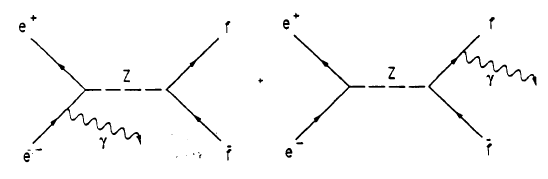
\includegraphics[width=0.75\linewidth]{graphics/Bremsstrahlungskorrektur}
	\end{figure}
	\begin{center}
	\begin{minipage}{0.4\linewidth}
			\begin{figure}
				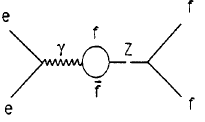
\includegraphics[width=0.8\linewidth]{graphics/presentationvertexschleifen}
			\end{figure}
	\end{minipage}
	\begin{minipage}{0.4\linewidth}
	\begin{figure}
			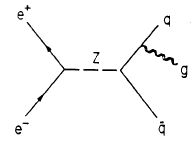
\includegraphics[width=0.8\linewidth]{graphics/presentation_QCDkorrektur}
	\end{figure}
	\end{minipage}
	\end{center}
\end{frame}

\subsection{Wirkungsquerschnitt und Zerfallsbreite}
\begin{frame}
	\frametitle{Wirkungsquerschnitt}
	\hspace{1cm} Ereignisrate bei Luminosität $L$:
	\begin{equation*}
	\scalebox{1.5}{$\dot{N} = \sigma \cdot L$}
	\end{equation*}
	\hspace{1cm} Wirkungsquerschnitt messen:
	\begin{equation*}
	\scalebox{1.5}{$\sigma = \frac{N}{\int L~\text{d}t}$}
	\end{equation*}
\end{frame}
\subsection{Vorwärts Rückwärts Asymmetrie}
\begin{frame}
	\frametitle{Vorwärts Rückwärts Asymmetrie}
	\begin{center}
		\begin{equation*}
		\sigma_f=\int_{0}^{1}\frac{\text{d}\sigma}{\text{d}cos(\theta)}~\text{d}cos(\theta)
		\end{equation*}
		\begin{equation*}
		\sigma_b=\int_{-1}^{0}\frac{\text{d}\sigma}{\text{d}cos(\theta)}~\text{d}cos(\theta)
		\end{equation*}
		\\
		\begin{equation*}
		\textcolor{lightgray}{A_{fb}=\frac{\sigma_f-\sigma_b}{\sigma_f+\sigma_b}}
		\end{equation*}
	\end{center}
\end{frame}
\begin{frame}
	\frametitle{Vorwärts Rückwärts Asymmetrie}
	\begin{center}
		\begin{equation*}
		\textcolor{lightgray}{\sigma_f=\int_{0}^{1}\frac{\text{d}\sigma}{\text{d}cos(\theta)}~\text{d}cos(\theta)}
		\end{equation*}
		\begin{equation*}
		\textcolor{lightgray}{\sigma_b=\int_{-1}^{0}\frac{\text{d}\sigma}{\text{d}cos(\theta)}~\text{d}cos(\theta)}
		\end{equation*}
		\\
		\begin{equation*}
		A_{fb}=\frac{\sigma_f-\sigma_b}{\sigma_f+\sigma_b}
		\end{equation*}
	\end{center}
\end{frame}
\begin{frame}
	\frametitle{Vorwärts Rückwärts Asymmetrie}
	\begin{center}
		Für Leptonen am Resonanzpeak:
		\begin{equation*}
		A_{fb}^{\ell,peak}\approx 3 \left ( \frac{g^{\ell}_V}{g^{\ell}_A} \right )^2=3\cdot (1-4 sin^2(\theta_w))
		\end{equation*}
	\end{center}
\end{frame}

\section{LEP und der OPAL Detektor}
\subsection{LEP am CERN}
%LEP luftaufnahme
\begin{frame}
	\frametitle{Der LEP Speicherring}
	\begin{figure}
		\includegraphics[width=1.0\linewidth]{graphics/LEPmap}
	\end{figure}
\end{frame}

\subsection{Der OPAL Detektor}
\begin{frame}
	\frametitle{Schematischer Aufbau}
	\begin{center}
	\begin{figure}
		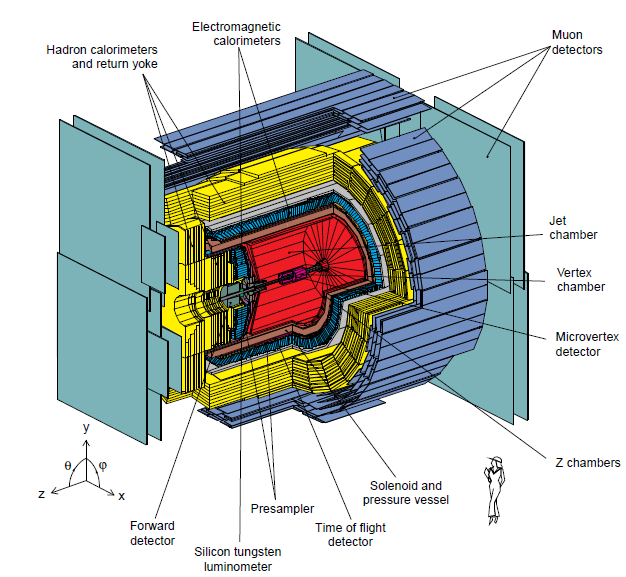
\includegraphics[width=0.7\linewidth]{graphics/OPALaufbau}
	\end{figure}
	\end{center}
\end{frame}

\begin{frame}
	\frametitle{Driftkammer}
	\begin{center}
		\begin{figure}
			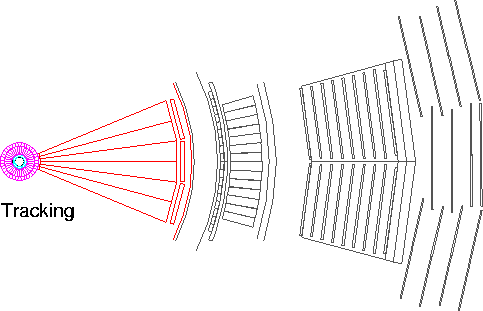
\includegraphics[width=0.75\linewidth]{graphics/slice_tracking_tr}
		\end{figure}
	\end{center}
\end{frame}

\begin{frame}
	\frametitle{Elektromagnetisches und hadronisches Kalorimeter}
	\begin{center}
		\begin{figure}
			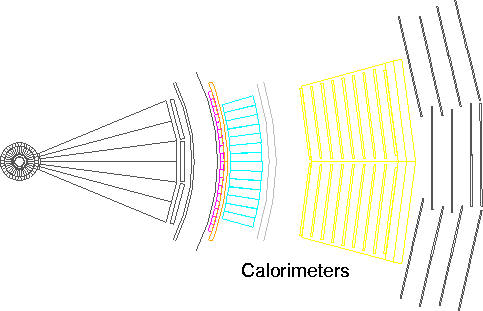
\includegraphics[width=0.75\linewidth]{graphics/slice_calorimeter_tr}
		\end{figure}
	\end{center}
\end{frame}

\begin{frame}
	\frametitle{Myonenkammer}
	\begin{center}
		\begin{figure}
			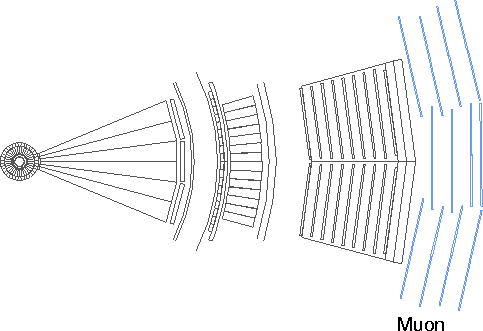
\includegraphics[width=0.75\linewidth]{graphics/slice_muon_tr}
		\end{figure}
	\end{center}
\end{frame}




\section{Datenanalyse}
\subsection{Detektor Bilder}
\begin{frame}
	\frametitle{Elektronen Events}
	\begin{minipage}{0.54\linewidth}
		\begin{figure}
			\centering
			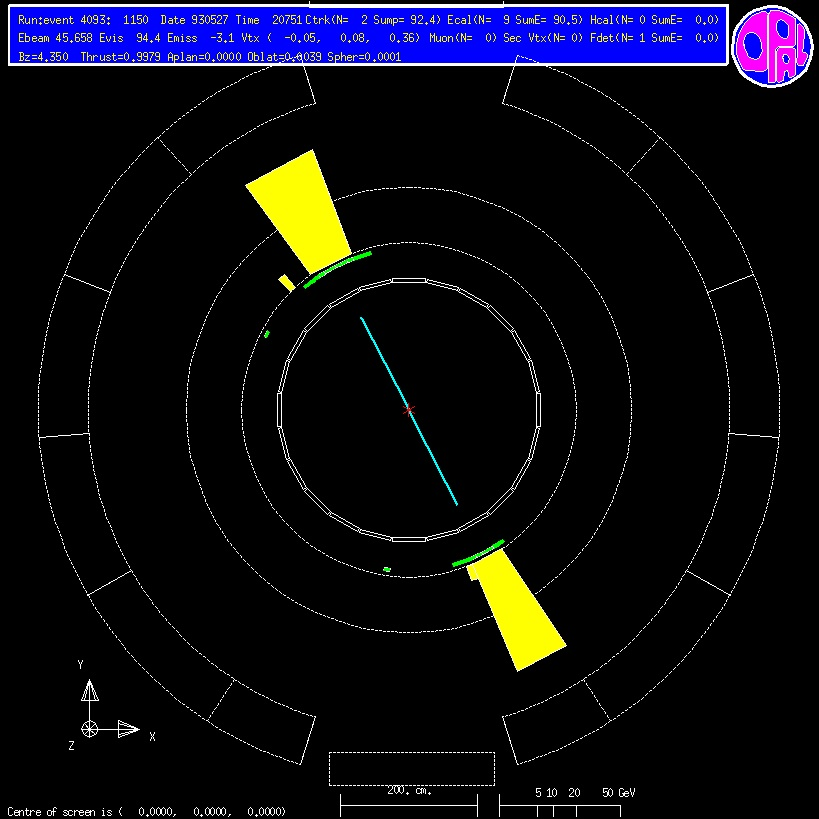
\includegraphics[width=1.0\linewidth]{graphics/electronopal}
		\end{figure}
	\end{minipage}
	\begin{minipage}{0.44\linewidth}
		\begin{center}
			\begin{itemize}
				\item 2 geladene Spuren\\\hfill
				\item Energie in EM-Kalorimeter\\\hfill
			\end{itemize}
		\end{center}
	\end{minipage}
\end{frame}

\begin{frame}
	\frametitle{Myonen Events}
		\begin{minipage}{0.54\linewidth}
			\begin{figure}
				\centering
				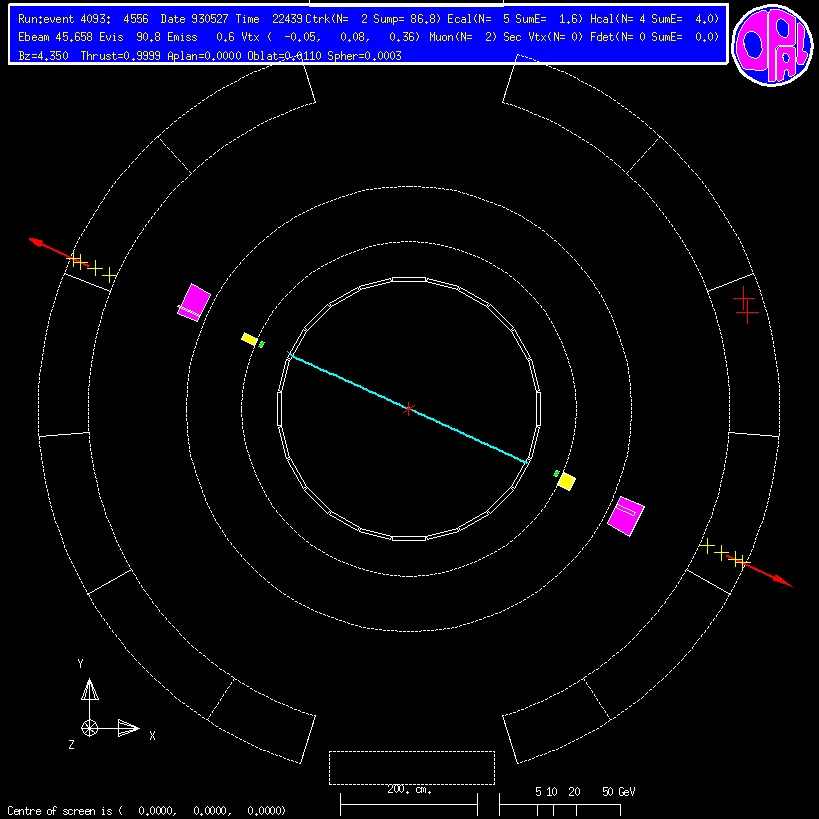
\includegraphics[width=1.0\linewidth]{graphics/muonopal}
			\end{figure}
		\end{minipage}
		\begin{minipage}{0.44\linewidth}
			\begin{center}
				\begin{itemize}
					\item 2 geladene Spuren\\\hfill
					\item Wenig Energie in EM-Kalorimeter\\\hfill
					\item Wenig Energie in Hadronenkalorimeter\\\hfill
					\item Spuren in Myonenkammer
				\end{itemize}
			\end{center}
		\end{minipage}
\end{frame}

\begin{frame}
	\frametitle{Leptonisches Tauonen Event}
		\begin{minipage}{0.54\linewidth}
			\begin{figure}
				\centering
				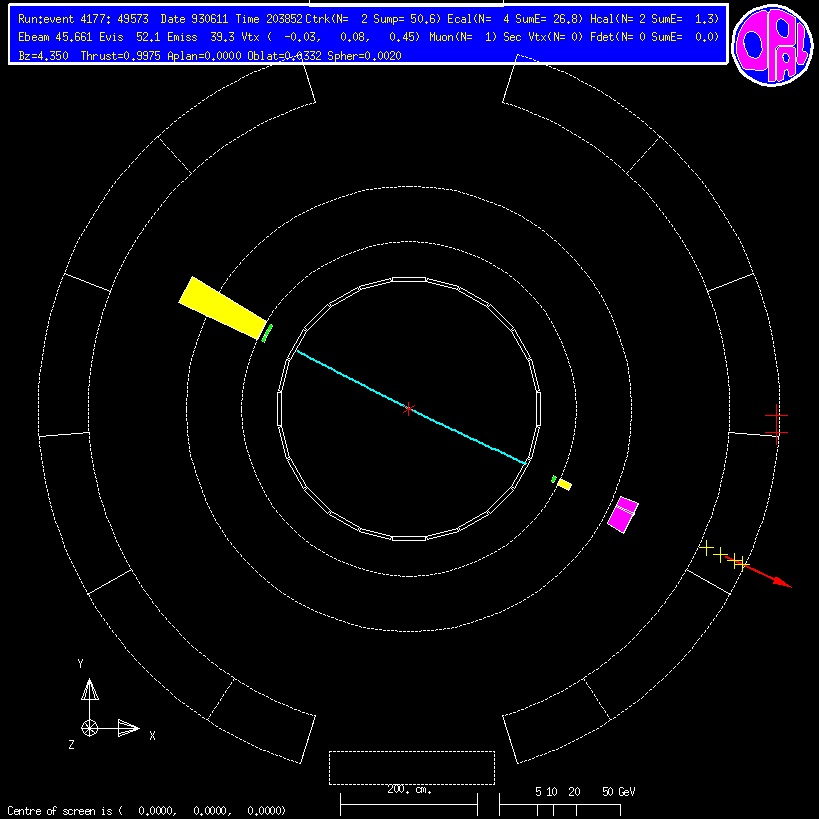
\includegraphics[width=1.0\linewidth]{graphics/tauonopalleptonisch}
			\end{figure}
		\end{minipage}
		\begin{minipage}{0.44\linewidth}
			\begin{center}
				\begin{itemize}
					\item Etwa $\frac{1}{3}$ Wahrscheinlichkeit\\\hfill
					\item 2 geladene Spuren\\\hfill
					\item Ein Myon, ein Elektron\\\hfill
				\end{itemize}
			\end{center}
		\end{minipage}
\end{frame}

\begin{frame}
	\frametitle{Hadronisches Tauonen Event}
		\begin{minipage}{0.54\linewidth}
			\begin{figure}
				\centering
				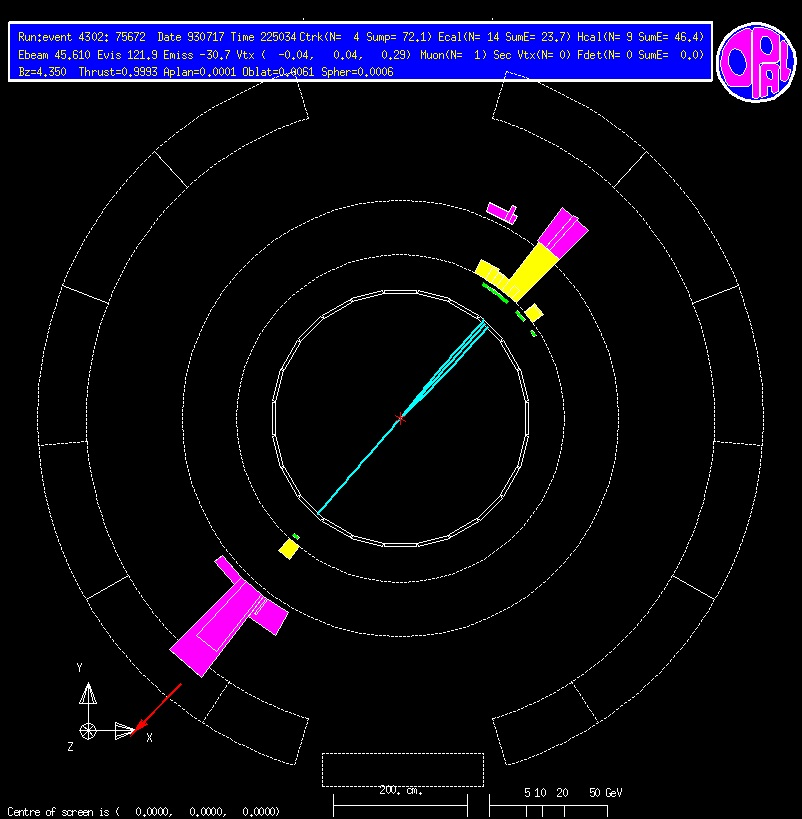
\includegraphics[width=1.0\linewidth]{graphics/tauonopalhadronisch}
			\end{figure}
		\end{minipage}
		\begin{minipage}{0.44\linewidth}
			\begin{center}
				\begin{itemize}
					\item Etwa $\frac{2}{3}$ Wahrscheinlichkeit\\\hfill
					\item Hier zwei mal drei Pionen\\\hfill
					\item Energie in beiden Kalorimetern\\\hfill
				\end{itemize}
			\end{center}
		\end{minipage}
\end{frame}


\begin{frame}
	\frametitle{Quark Events}
		\begin{minipage}{0.54\linewidth}
			\begin{figure}
				\centering
				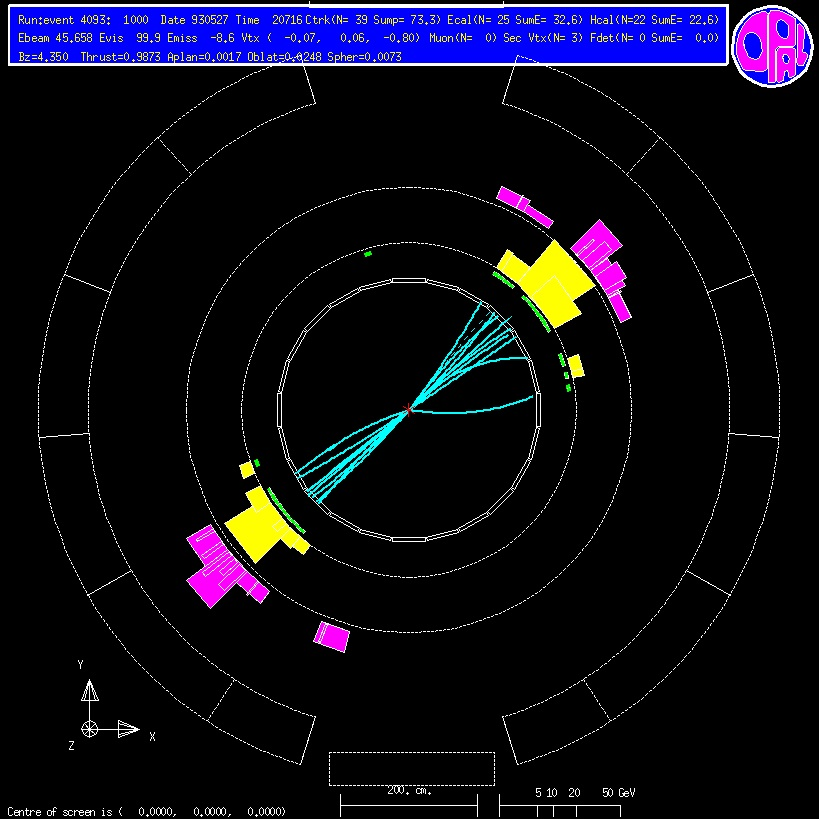
\includegraphics[width=1.0\linewidth]{graphics/quarkopal}
			\end{figure}
		\end{minipage}
		\begin{minipage}{0.44\linewidth}
			\begin{center}
				\begin{itemize}
					\item Ähnlichkeit mit Hadr. Tauonen\\\hfill
					\item Sehr viele Spuren\\\hfill
					\item Energie in beiden Kalorimetern\\\hfill
					\item Beugung der Kurven wegen Magnetfeld
				\end{itemize}
			\end{center}
		\end{minipage}
\end{frame}



\subsection{Cuts und Aufbereitung der Daten}
\begin{frame}
	\frametitle{MC-Simulationen}
	\begin{center}
		\begin{itemize}
			\item Zu viele Events um einzeln zu unterscheiden\\\hfill
			\item Events an Variablen (E\_Ecal, Ncharged...) unterscheiden\\\hfill
			\item MC-Simulation von Events und Detektorsimulation\\\hfill
			\item Daraus Weg finden, Events zu trennen
		\end{itemize}
	\end{center}	
\end{frame}
\begin{frame}
	\frametitle{Energie im EM Kalorimeter}
	\begin{figure}
		\centering
		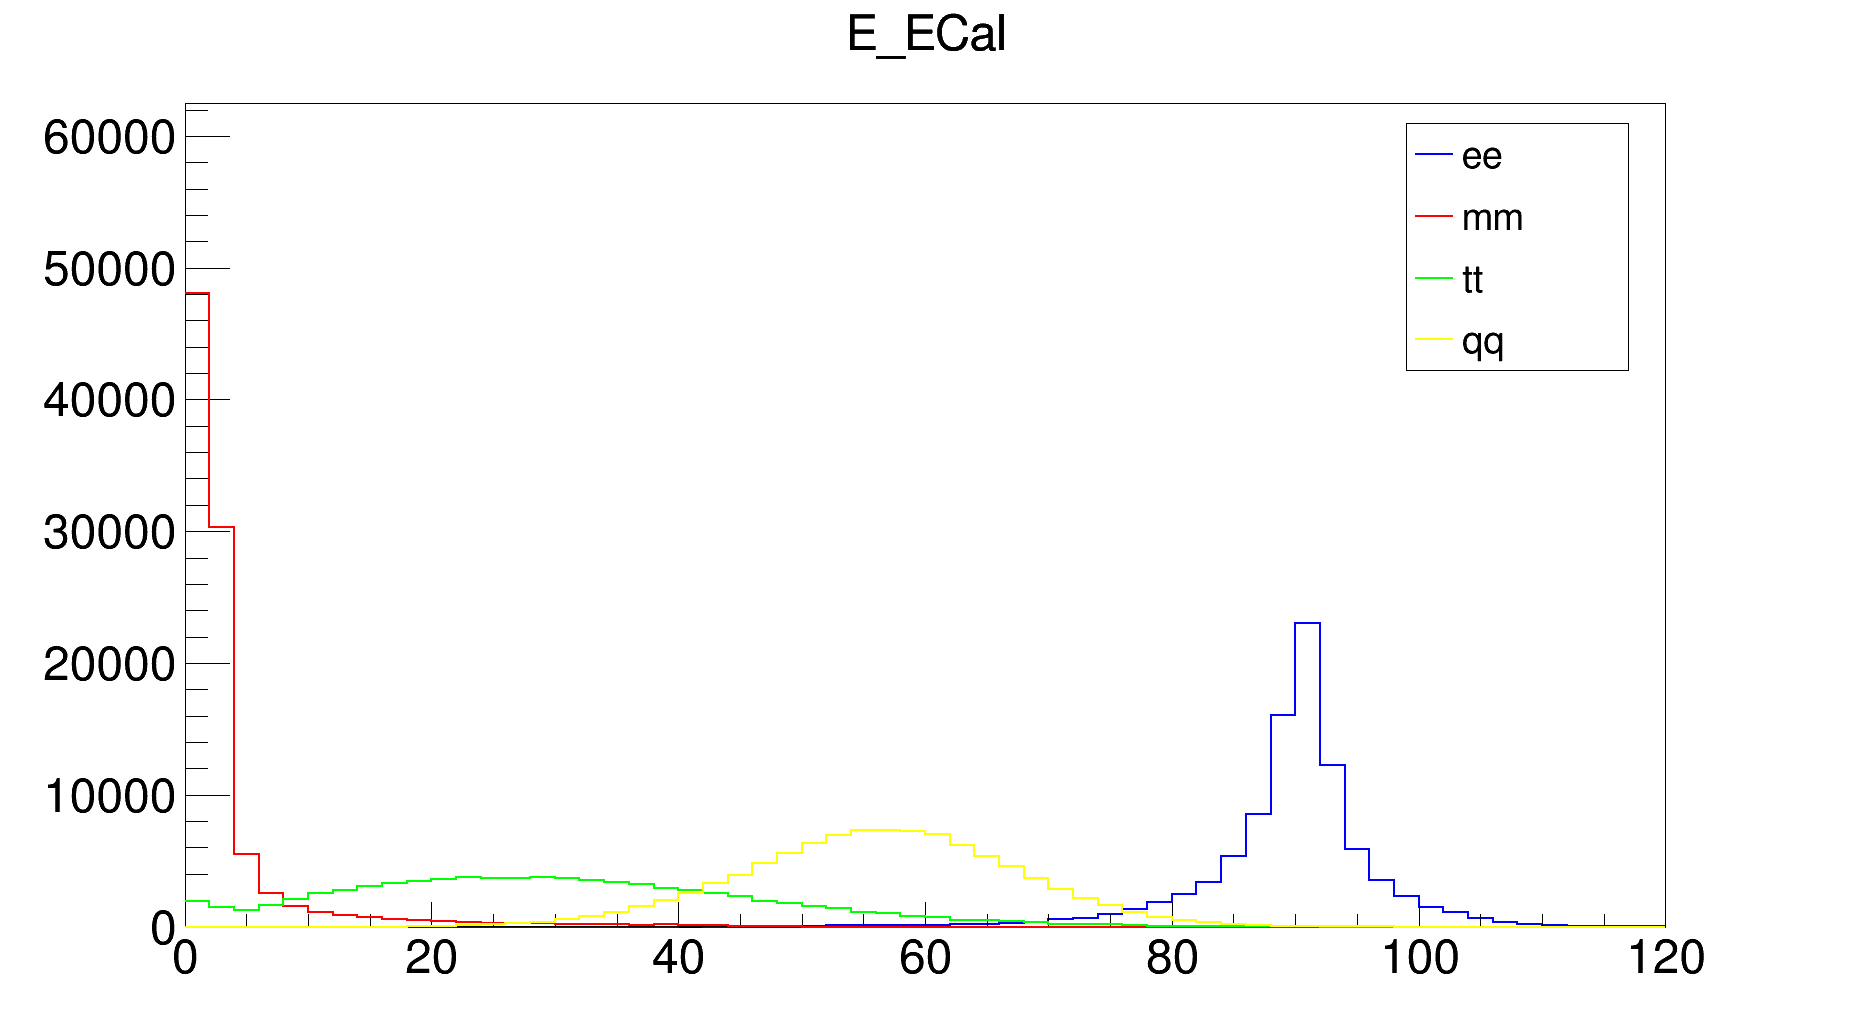
\includegraphics[width=0.9\linewidth]{../results/MC_results/nocut/E_Ecal}
	\end{figure}
	\begin{center}
		\begin{itemize}
			\item \makebox[3cm][l]{\textbf{Elektronen Cut:}} $\ge 70 \unit{GeV}$
			\item \makebox[3cm][l]{\textbf{Myonen Cut:}} $< 50 \unit{GeV}$
			\item \makebox[3cm][l]{\textbf{Tauonen Cut:}} $< 60 \unit{GeV}$
		\end{itemize}
	\end{center}
\end{frame}

\begin{frame}
	\frametitle{Anzahl der geladenen Spuren}
	\begin{figure}
		\centering
		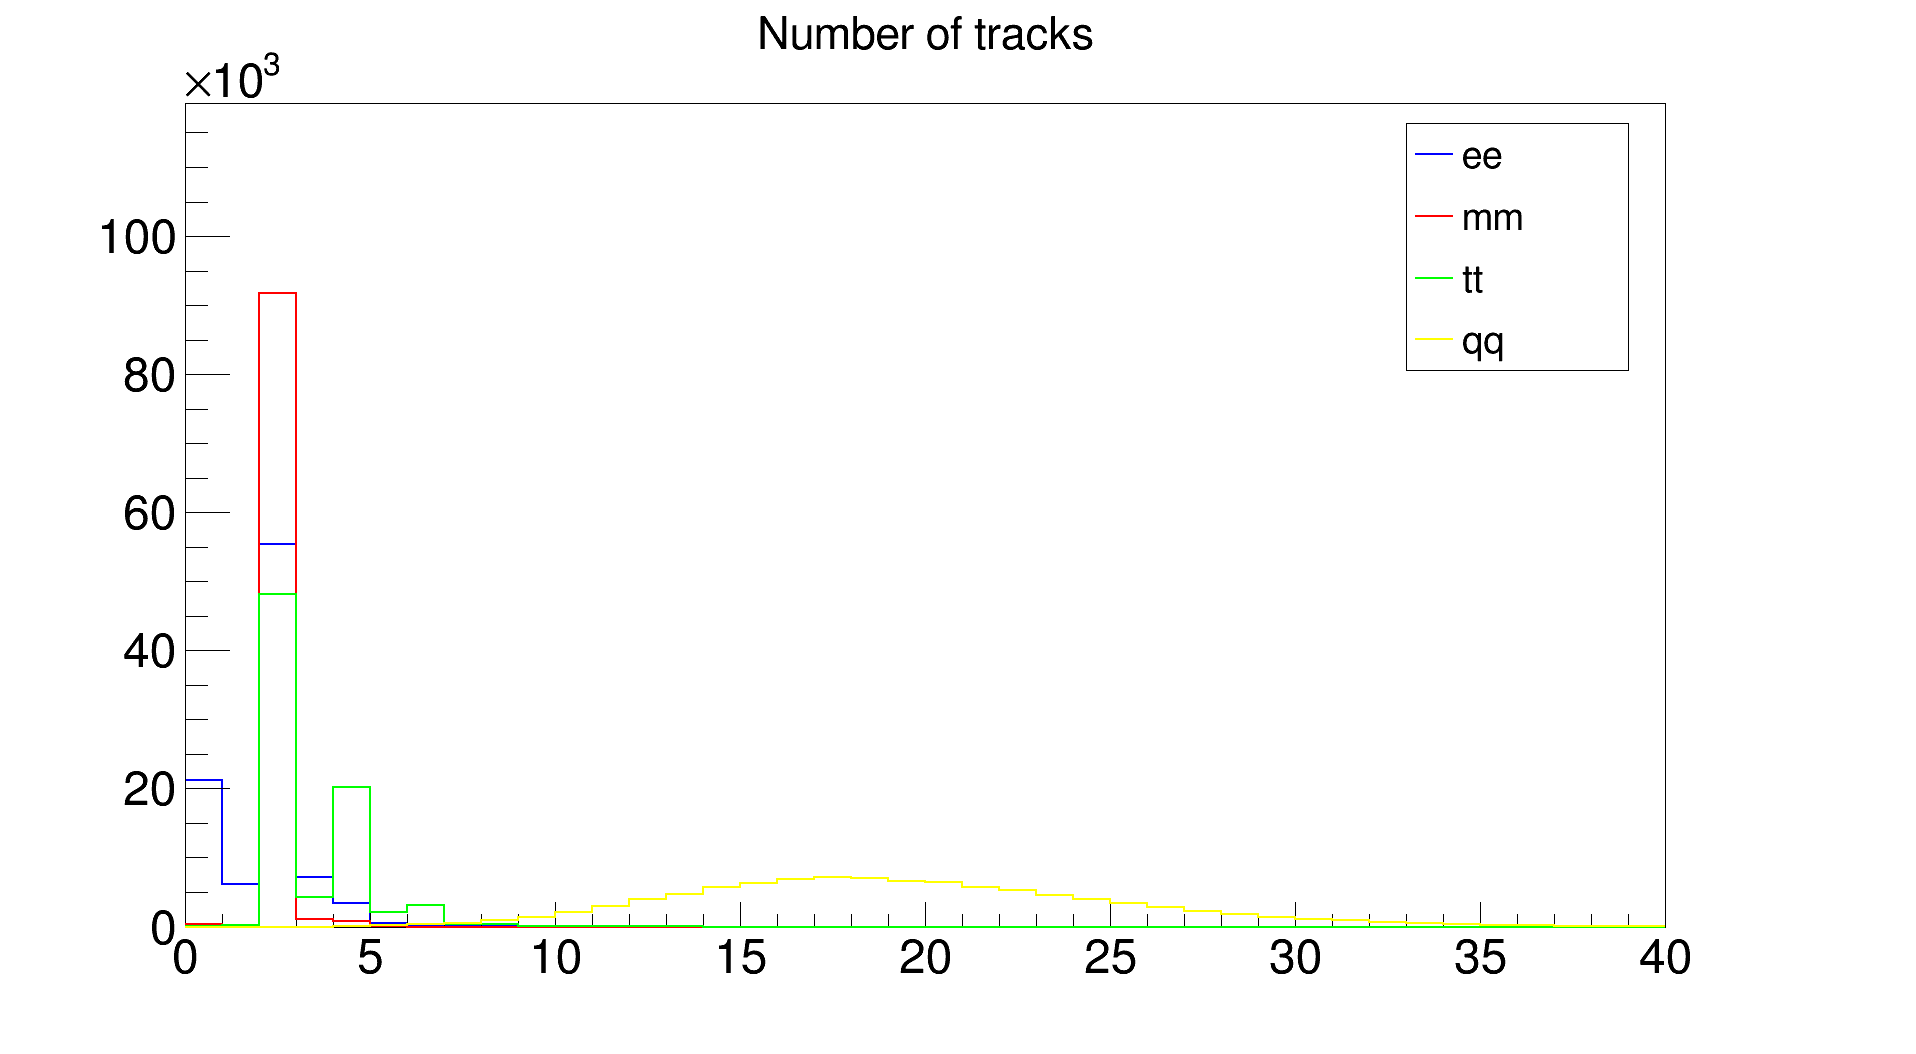
\includegraphics[width=0.85\linewidth]{../results/MC_results/nocut/Ncharged}
	\end{figure}
	\begin{center}
		\begin{itemize}
			\item \makebox[3cm][l]{\textbf{Elektronen Cut:}} $<7$
			\item \makebox[3cm][l]{\textbf{Myonen Cut:}} $=2$
			\item \makebox[3cm][l]{\textbf{Tauonen Cut:}} $<7$
			\item \makebox[3cm][l]{\textbf{Quark Cut:}} $\ge8$
		\end{itemize}
	\end{center}
\end{frame}

\begin{frame}
	\frametitle{Vorher-Nacher Vergleich}
	\begin{minipage}{0.48\linewidth}
			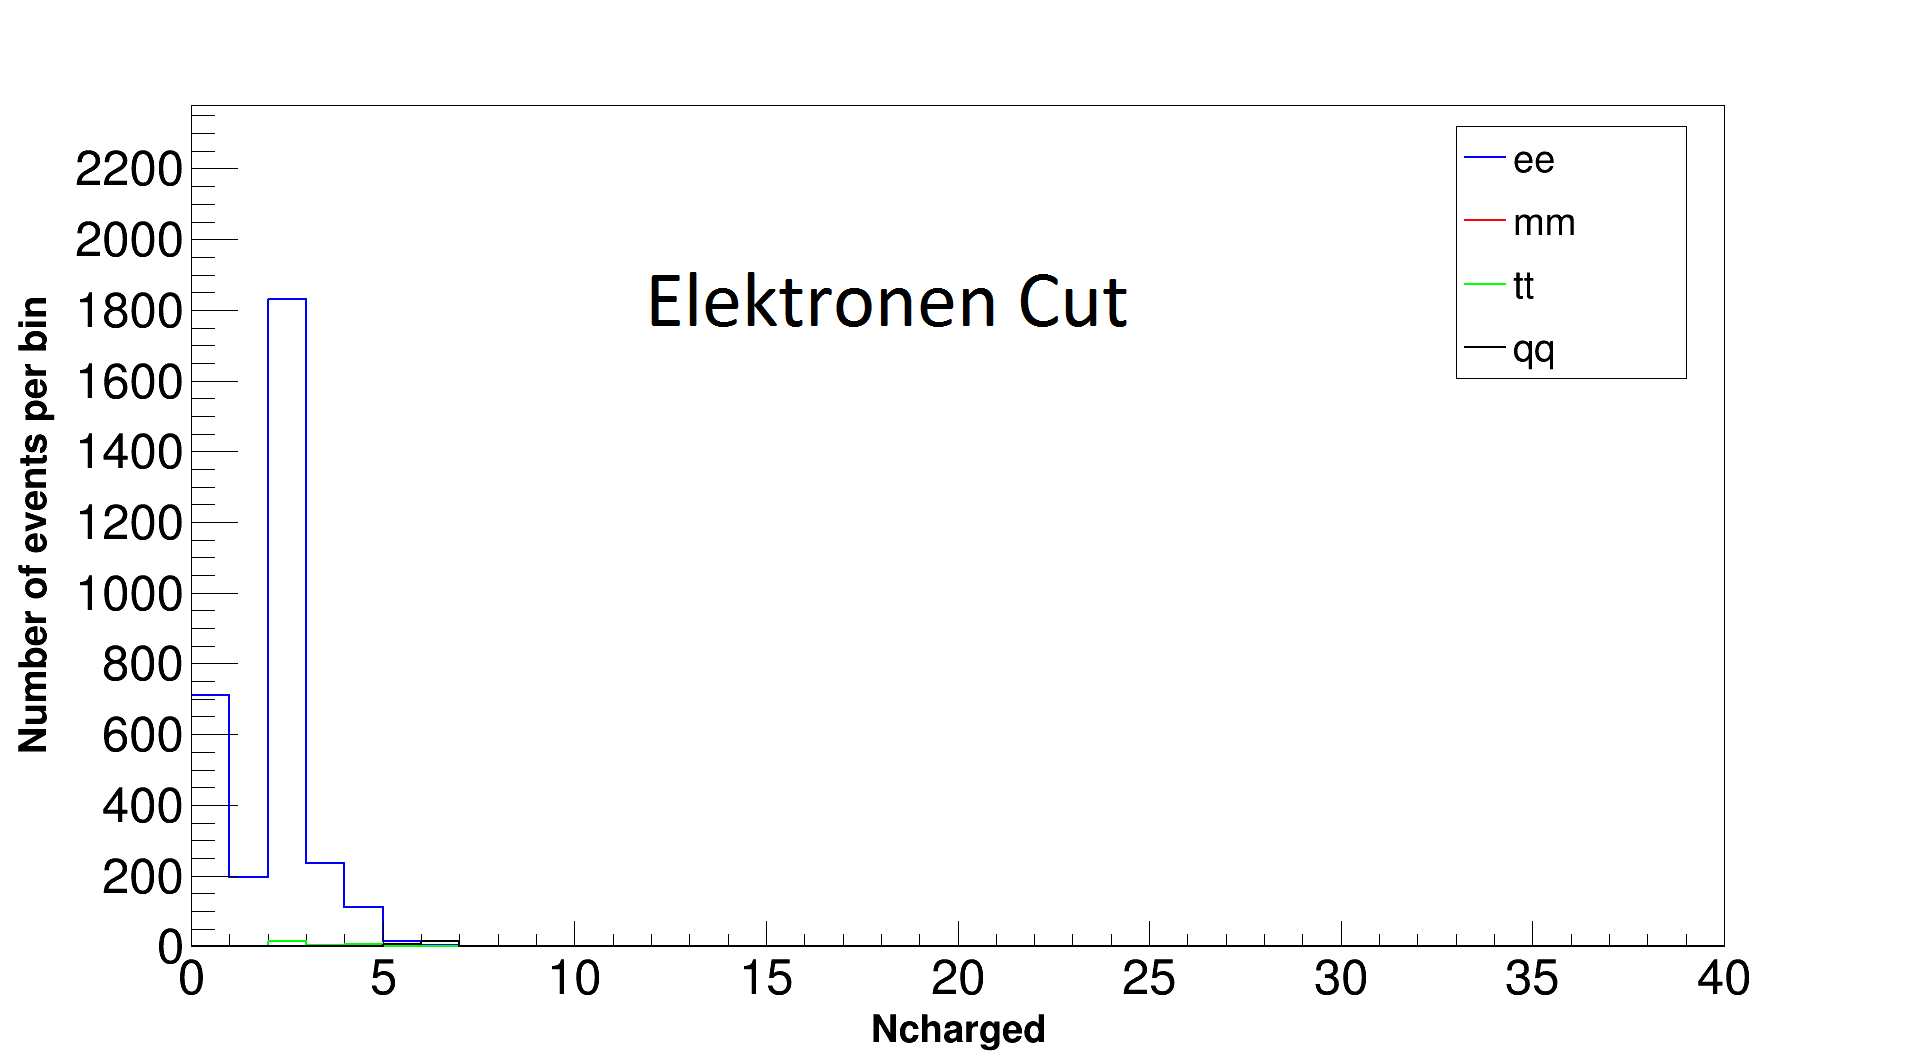
\includegraphics[width=1.1\linewidth]{graphics/Ncharged_vergleich_ee}\\
			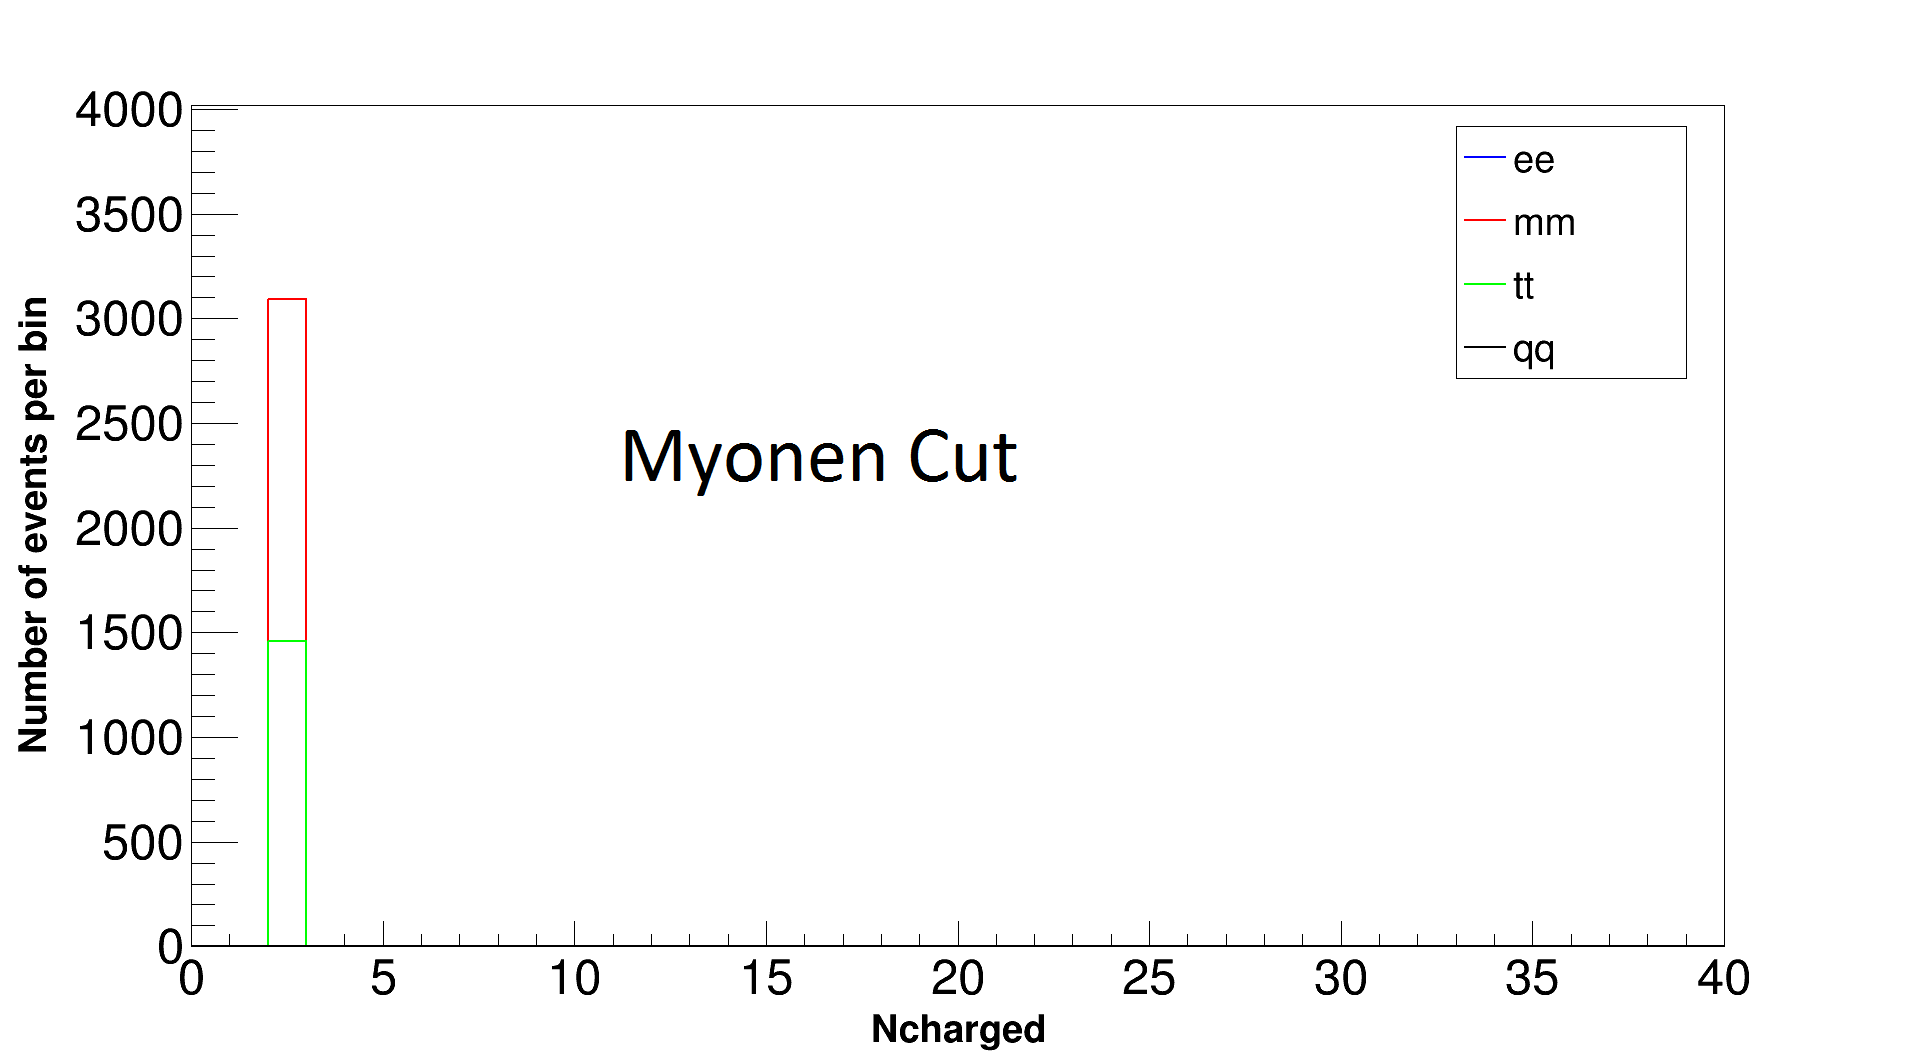
\includegraphics[width=1.1\linewidth]{graphics/Ncharged_vergleich_mm}
	\end{minipage}
	\begin{minipage}{0.48\linewidth}
			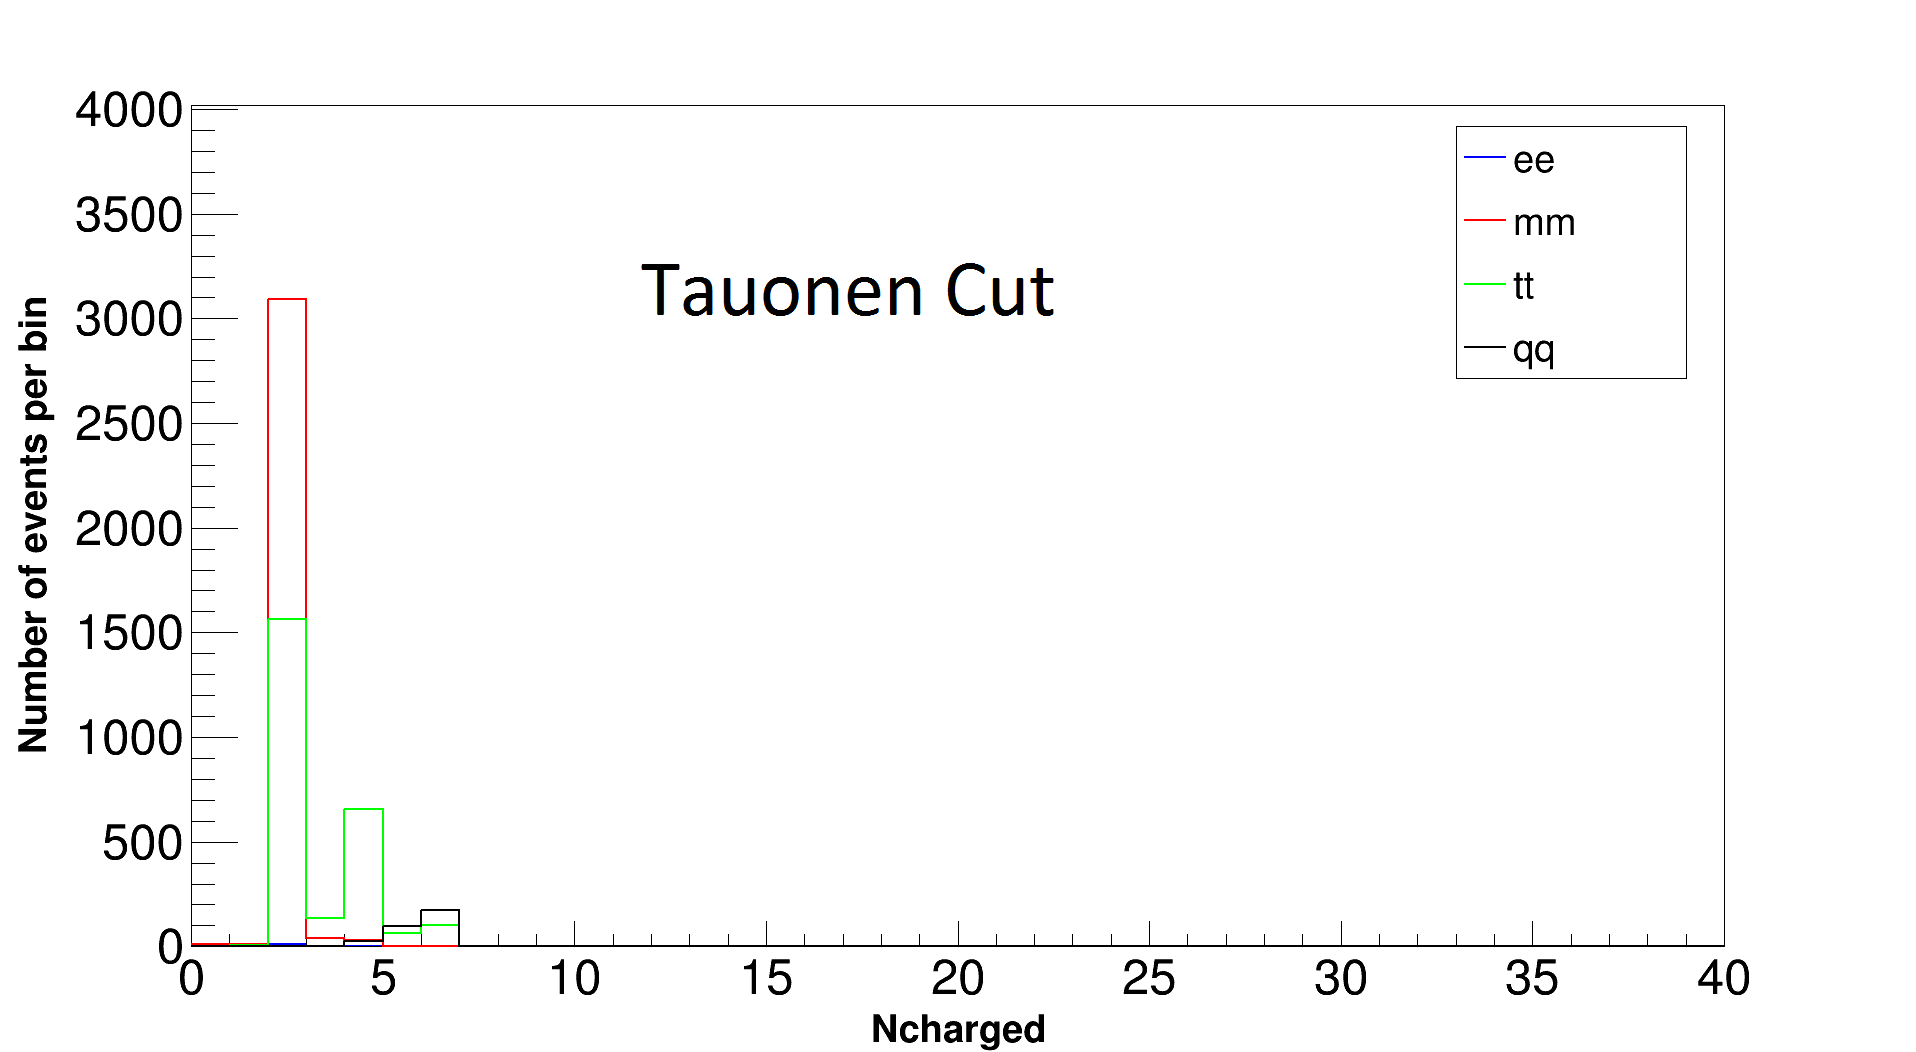
\includegraphics[width=1.1\linewidth]{graphics/Ncharged_vergleich_tt}\\
			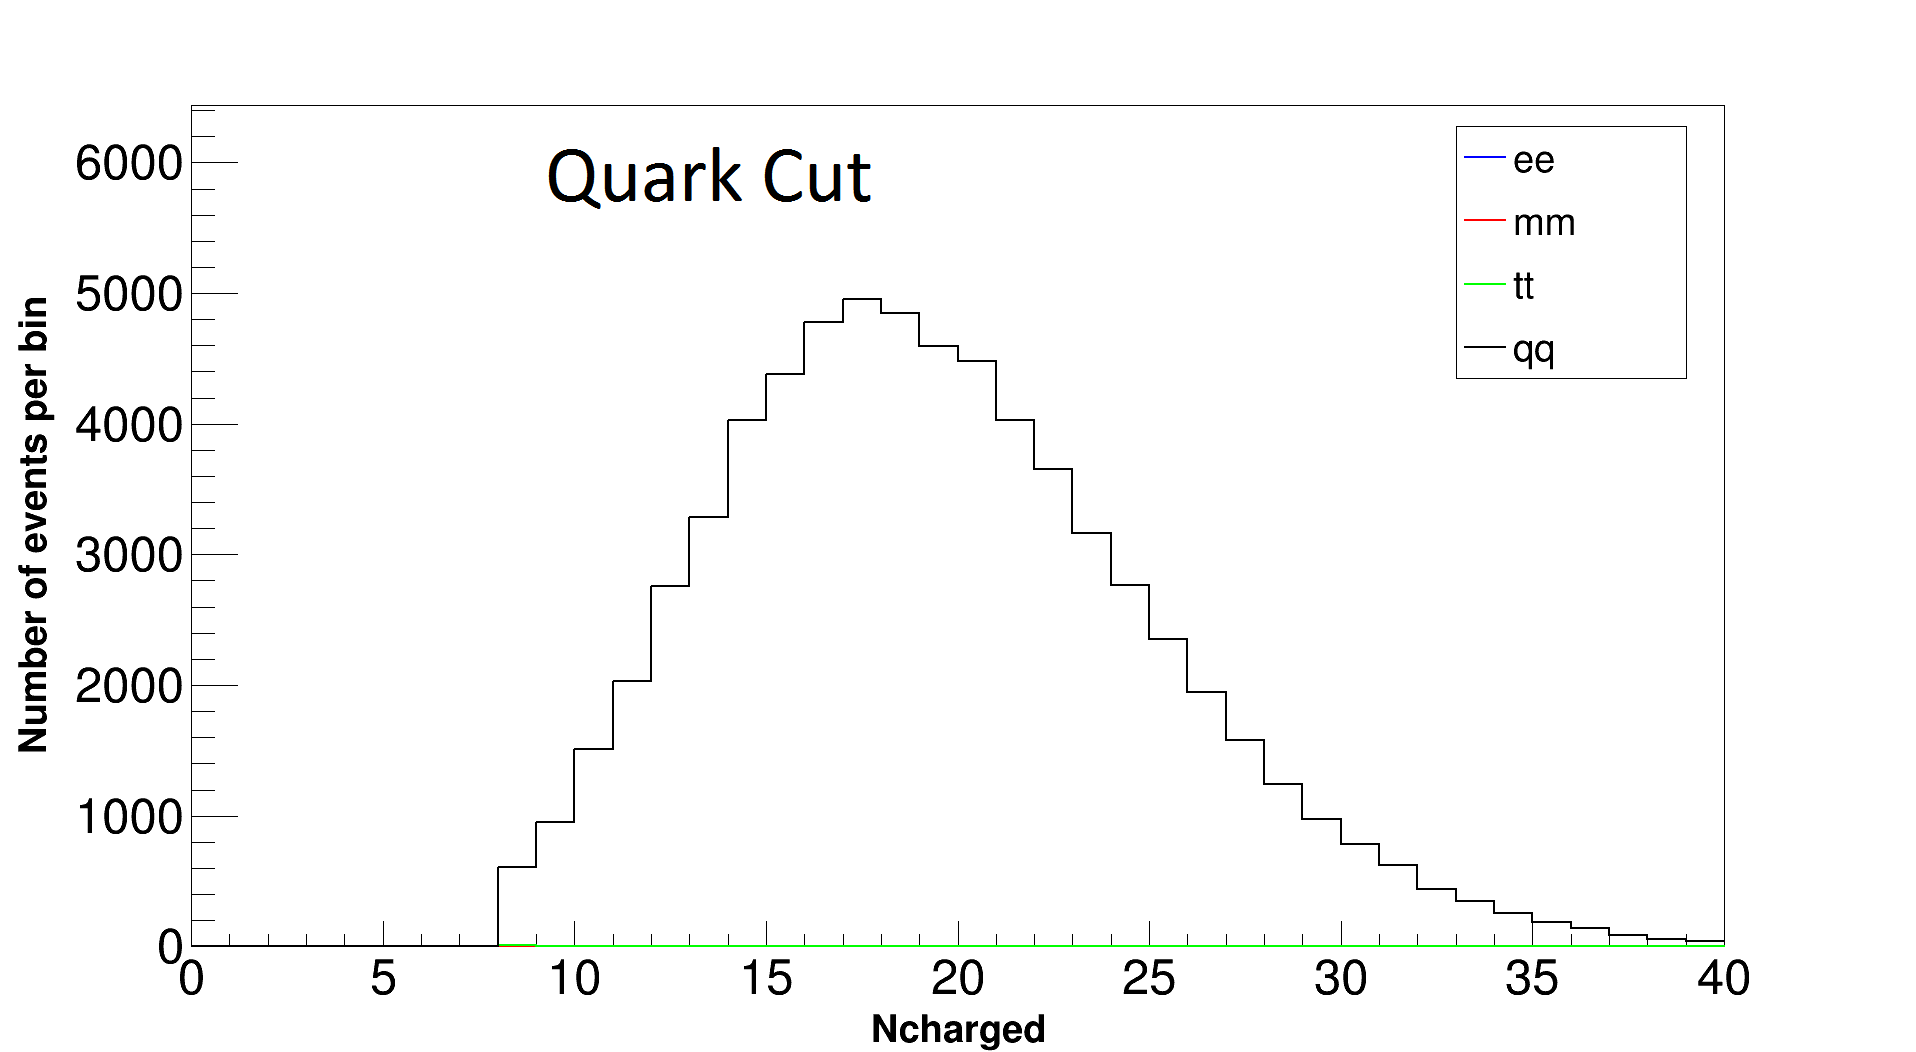
\includegraphics[width=1.1\linewidth]{graphics/Ncharged_vergleich_qq}
		\end{minipage}
\end{frame}
\begin{frame}
	\frametitle{Übersicht über die Cuts}
	\begin{table}[H]\centering
		\begin{tabular}{@{}llllll@{}}
			\toprule
			&			&Ncharged	&Pcharged [GeV]	&E\_Ecal [GeV] &Cos\_theta\\ 
			\midrule
			&$e^+e^-$	&$<7$		&				&$\ge70$		&$\ge-0.9$ \& $\le0.9$\\
			&$\mu^+\mu^-$		&$=2$			&$>71$		&$<50$			&			\\
			&$\tau^+\tau^-$		&$<7$		&$\le60$			&$<60$			&					\\
			&$q\overline{q}$		&$\ge8$		&				&				&			\\
			\bottomrule
		\end{tabular}
	\end{table}
	\begin{minipage}{0.48\linewidth}
		\centering
		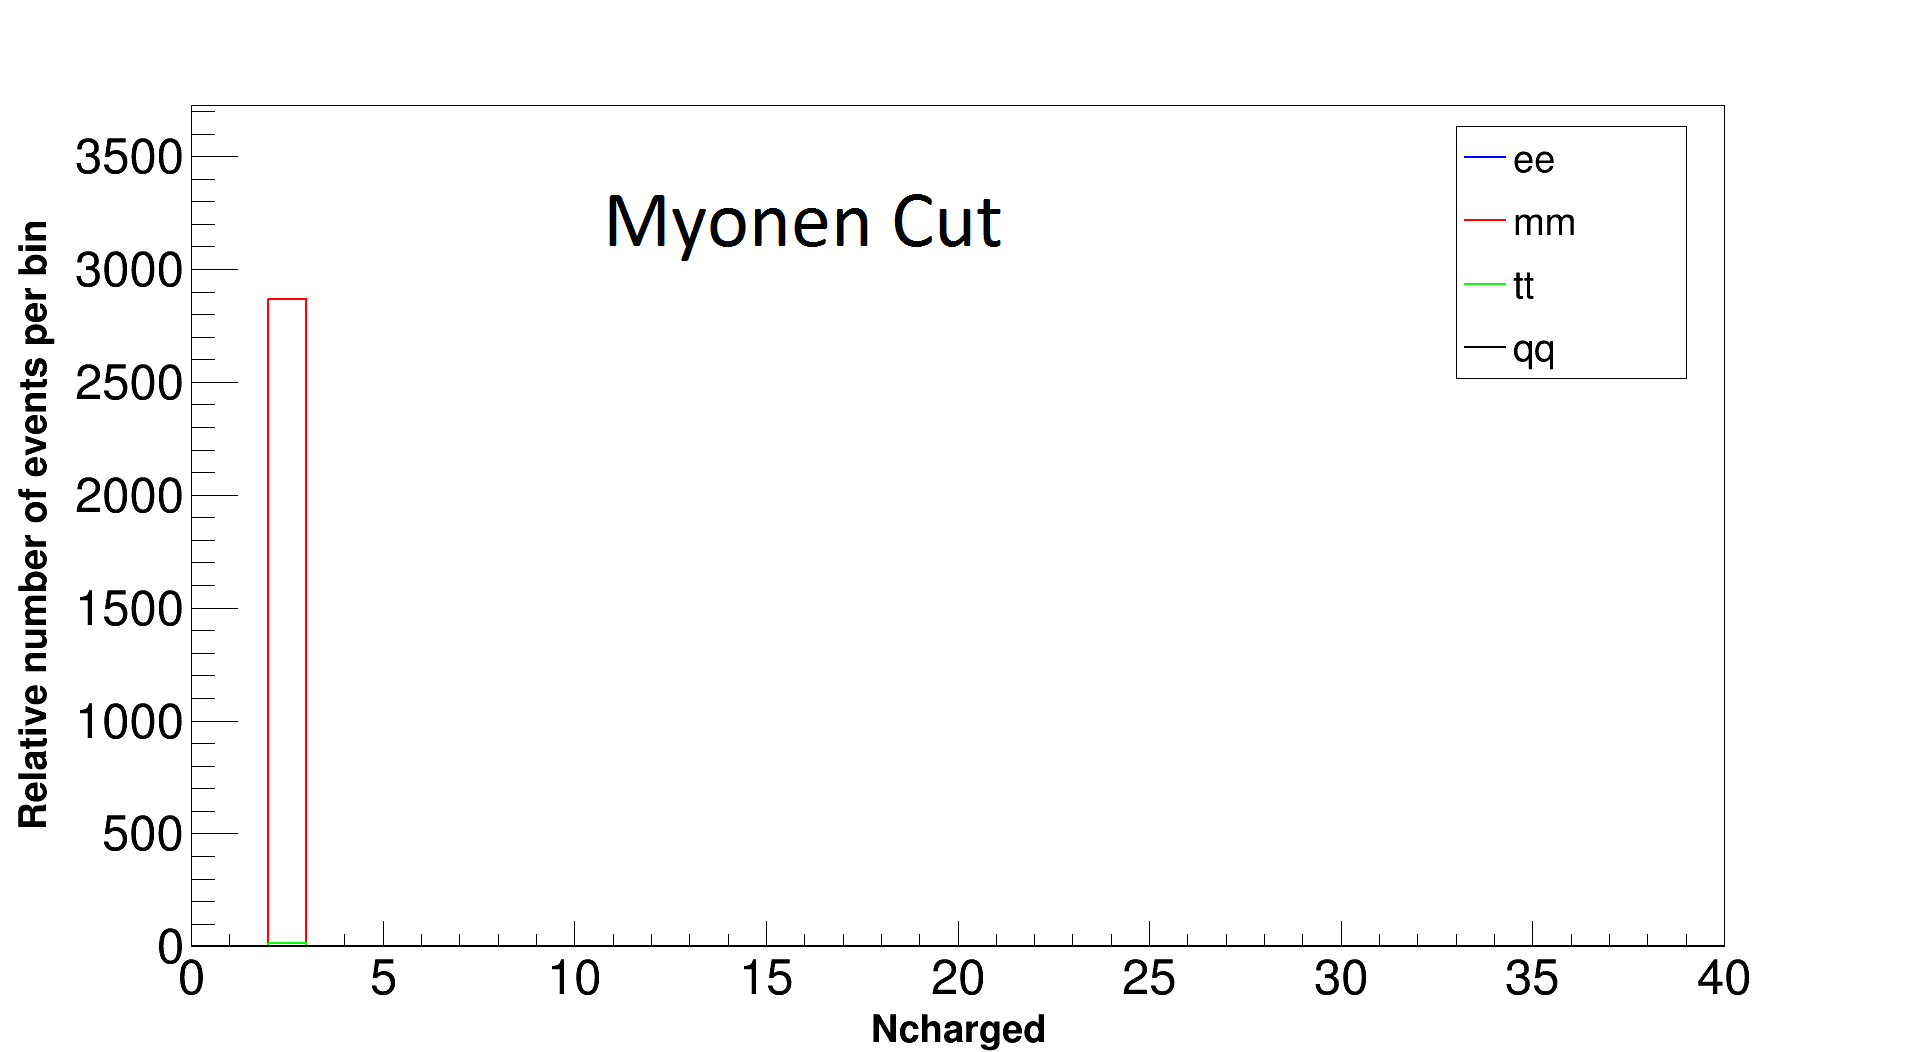
\includegraphics[width=1.1\linewidth]{graphics/Ncharged_final_mm}
	\end{minipage}
	\begin{minipage}{0.48\linewidth}
		\centering
		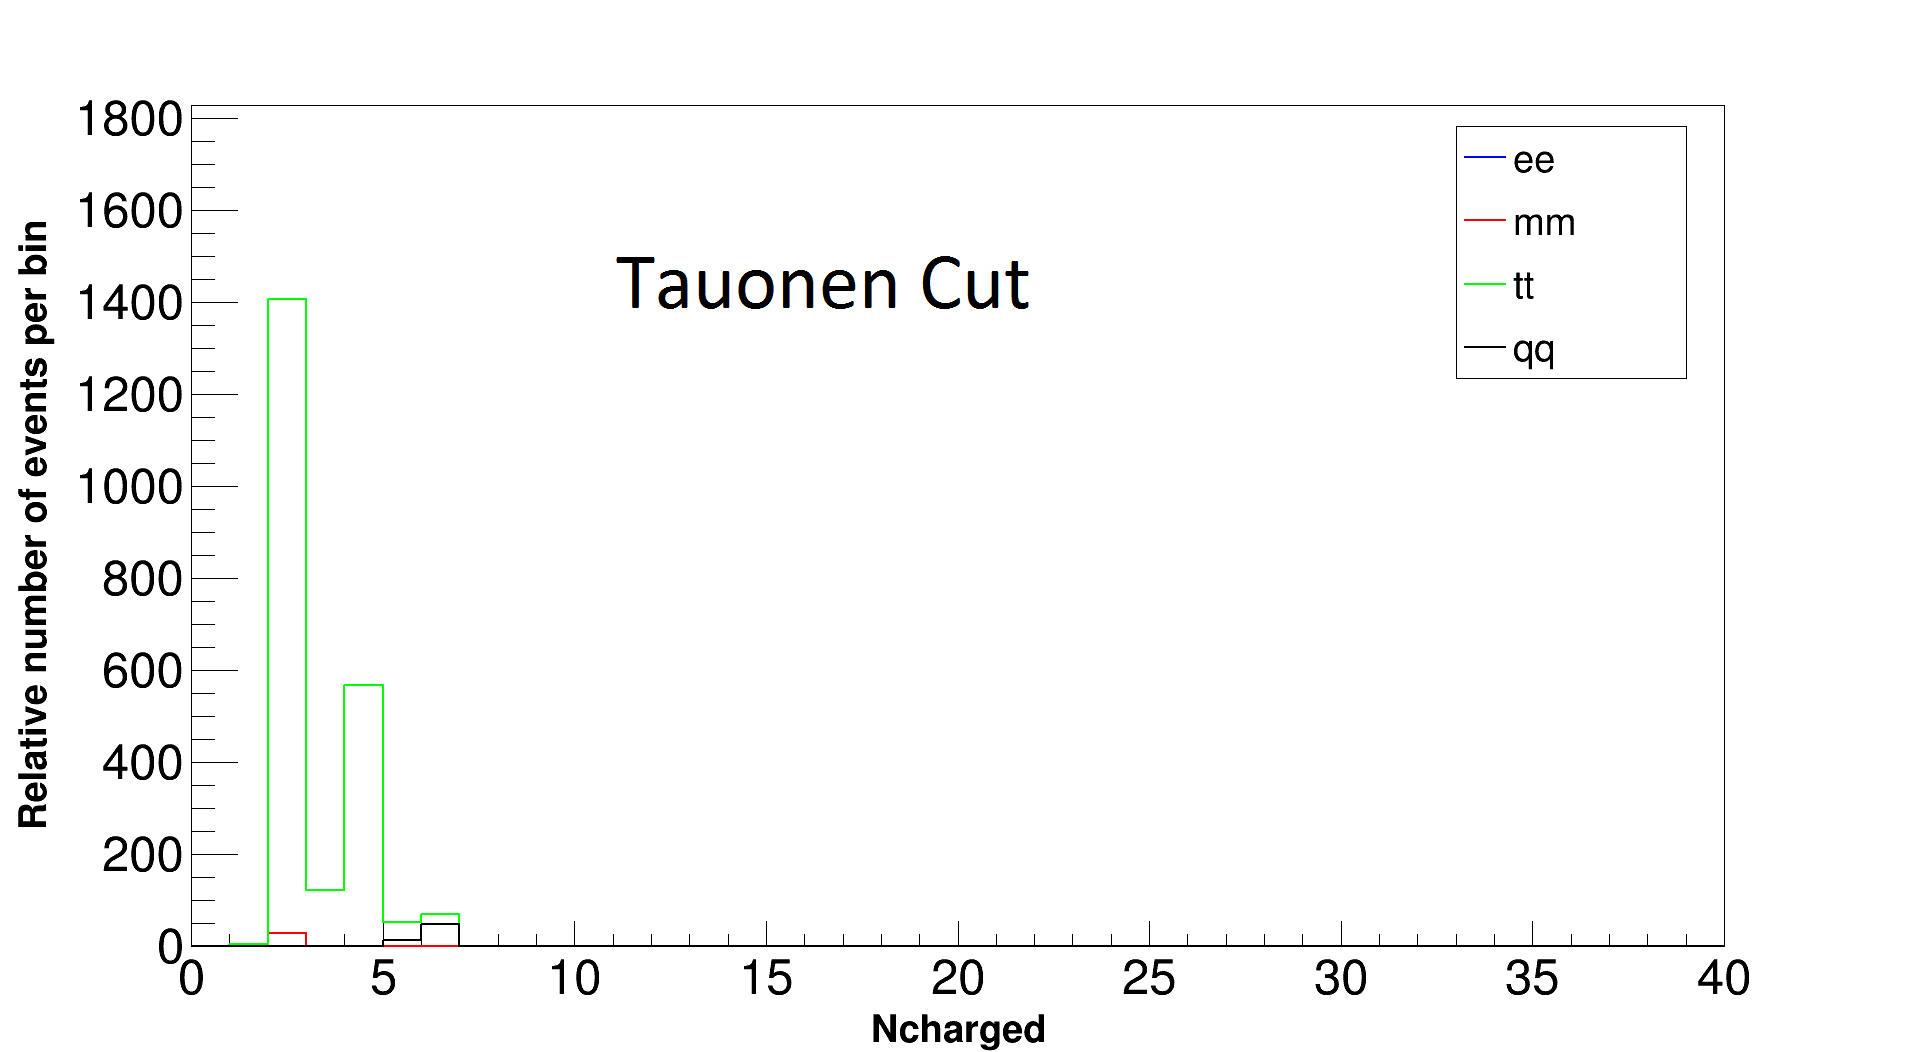
\includegraphics[width=1.1\linewidth]{graphics/Ncharged_final_tt}
	\end{minipage}
\end{frame}
\begin{frame}
	\frametitle{Zwei-Photonen Untergrund}
	\begin{minipage}{0.48\linewidth}
		\centering
		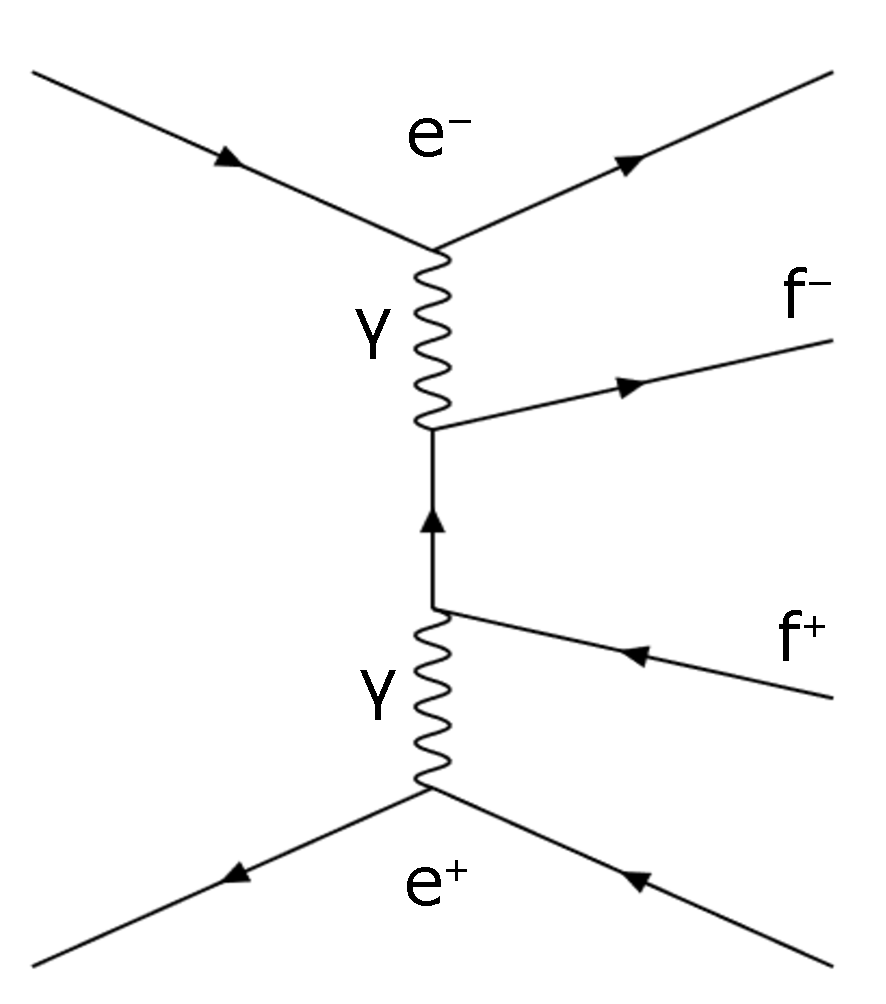
\includegraphics[width=1.0\linewidth]{graphics/twophotonfeynman}
	\end{minipage}
	\begin{minipage}{0.48\linewidth}
		\begin{center}
			\begin{itemize}
				\item Inelastisches Streuungsereignis\\\hfill
				\item Elektronen verlieren wenig Energie\\\hfill
				\item Kein $Z^0$ beteiligt \\$\Rightarrow$ Untergrund\\\hfill
				\item Niederenergetische Fermionen\\ $\Rightarrow$ Zusätzlicher Cut
			\end{itemize}
		\end{center}
	\end{minipage}
\end{frame}


\begin{frame}
	\frametitle{Die Effizienzmatrix}
	Anzahl ausgewählter Elektronenevents:
	\begin{equation*}
	C_e = E_{11} \cdot N_{e} + E_{12} \cdot N_\mu +E_{13} \cdot N_\tau+E_{14} \cdot N_q
	\end{equation*}
	\begin{equation*}
	E_{ij}=\frac{n^{cut}_{ij}}{N_i},\qquad \vec{C}=\boldsymbol{E}\cdot\vec{N}
	\end{equation*}
	\begin{table}[H]\centering
		\begin{tabular}{@{}llllll@{}}
			\toprule
			&Events &$e^+e^-$&$\mu^+\mu^-$&$\tau^+\tau^-$&$q\overline{q}$\\
			\midrule
			&Cut&&&&\\
			&$e^+e^-$&0.39078&0.00002&0.00422&0.00002\\
			&$\mu^+\mu^-$&0.00018&0.90171&0.00611&0.00001\\
			&$\tau^+\tau^-$&0.00039&0.00940&0.83413&0.00094\\
			&$q\overline{q}$&0.00007&0.00001&0.00685&0.98437\\
		\end{tabular}\\
		\noindent\textbox{\hfil Effizienzmatrix\hfil}
	\end{table}
\end{frame}

\begin{frame}
	\frametitle{Reinheit der Cuts}
	\hspace{2cm} Branching Ratios
	\begin{equation*}
		BR_i=\frac{\Gamma_i}{\sum_{j}\Gamma_{j}}
	\end{equation*}
	\hspace{2cm} Reinheit
	\begin{equation*}
		P_i=\frac{BR_i\cdot E_{ii}/N_i}{\sum_{j}BR_j\cdot E_{ij}/N_j}
	\end{equation*}
	\begin{table}\centering
		\begin{tabular}{@{}lll@{}}
			\toprule
			&Cut&Purity\\
			\midrule
			&$e^+e^-$&0.9882\\
			&$\mu^+\mu^-$&0.9928\\
			&$\tau^+\tau^-$&0.9661\\
			&$q\overline{q}$&0.9997\\
			\bottomrule
		\end{tabular}
	\end{table}
\end{frame}

\begingroup
\Large
\begin{frame}
	\frametitle{Die Inverse Effizienzmatrix}
	\hspace{2cm} Eigentliche Anzahl gesucht:
	\begin{equation*}
		\vec{N}=\boldsymbol{E}^{-1}\cdot\vec{C}=:\boldsymbol{I}\cdot\vec{C}
	\end{equation*}
	\hspace{2cm} Toy Experiments:
	\begin{equation*}
		E^{k}_{ij}=E_{ij}+G^k\cdot s_{E_{ij}}
	\end{equation*}
\end{frame}
\endgroup

\begin{frame}
	\frametitle{s-t-Kanal Trennung}
	\centering
	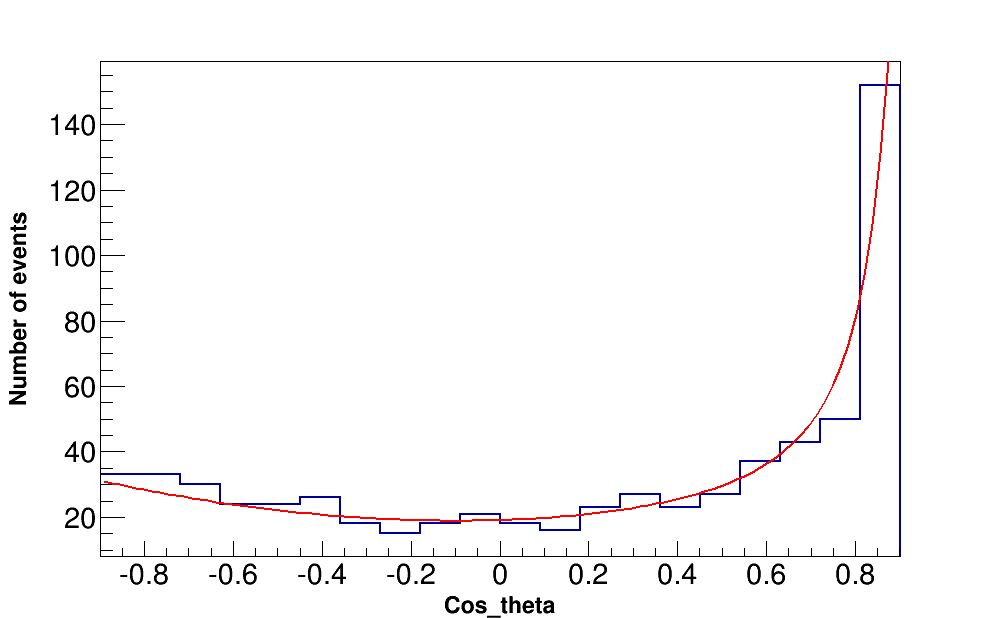
\includegraphics[width=0.85\linewidth]{../results/data_results/cosp_fits/stchannelexample46.png}
	\hspace{2cm} Fit Funktion $N(x)=A_s\cdot(1-x^2)+A_t\cdot(1-x)^{-2}$
\end{frame}

\begin{frame}
	\frametitle{Berechnung des Korrekturfaktors}
	\begin{minipage}{0.7\linewidth}
		\begin{equation*}
		c_{st}=\frac{A_s\int_{-0.9}^{0.9}(1+x^2)dx}{A_s\int_{-0.9}^{0.9}(1+x^2)dx+A_t\int_{-0.9}^{0.9}(1-x)^{-2}dx}
		\end{equation*}\\
		\hfill\\
		\hspace{2cm} Integrale sind konstant
		\begin{align*}
		\int_{-0.9}^{0.9}(1+x^2)dx&=2.286\\
		\int_{-0.9}^{0.9}(1-x)^{-2}dx&=9.474
		\end{align*}
	\end{minipage}
	\begin{minipage}{0.28\linewidth}
		\begin{tabular}{@{}lll@{}}
			\toprule
			&$\sqrt{s}$ [GeV]&$c_{st}$\\
			\midrule
			&$88.48$&0.12(2)\\
			&$89.47$&0.37(2)\\
			&$90.23$&0.52(2)\\
			&$91.23$&0.688(8)\\
			&$91.97$&0.66(2)\\
			&$92.97$&0.44(3)\\
			&$93.72$&0.47(3)\\
			\bottomrule
		\end{tabular}
	\end{minipage}
\end{frame}

\subsection{Auswertung der aufgearbeiteten Daten}
\begin{frame}
	\frametitle{Wirkungsquerschnitte Elektronen Cut}
	\centering
	\includegraphics[width=0.90\linewidth]{../results/data_results/wqs/WQee}
	\begin{equation*}
	\sigma_i=\frac{N_i}{L}+c_{beam,i}
	\end{equation*}
\end{frame}
\begin{frame}
	\frametitle{Wirkungsquerschnitte Tauonen Cut}
	\centering
	\includegraphics[width=0.90\linewidth]{../results/data_results/wqs/WQtt}
	\begin{itemize}
		\item Elektronen und Taunen Ergebnis nicht in Übereinstimmung mit theoretischem Wert für $\Gamma_l$
	\end{itemize}
\end{frame}
\begin{frame}
	\frametitle{Wirkungsquerschnitte Myonen Cut}
	\centering
	\includegraphics[width=0.90\linewidth]{../results/data_results/wqs/WQmm}
	\begin{itemize}
		\item In weiteren Rechnungen $\Gamma_l=\Gamma_\mu$, da s-t-Kanal und Quark-Tauonen Unterscheidung problematisch
	\end{itemize}
\end{frame}
\begin{frame}
	\frametitle{Wirkungsquerschnitte Quark Cut}
	\centering
	\includegraphics[width=0.90\linewidth]{../results/data_results/wqs/WQqq}
	\begin{equation*}
		\Gamma_q=\frac{\Gamma_f^2}{\Gamma_\mu}=(1777\pm41)\unit{MeV}
	\end{equation*}
\end{frame}
\begin{frame}
	\frametitle{Zerfallsbreiten und Leptonenuniversalität}
	\mbox{}\\
	\begin{equation*}
	\sigma(s) = \frac{12\pi}{ \tikzmark{MZ1}M_Z^2}\frac{s\cdot \tikzmark{gammaf}\Gamma_f^2}{(s-\tikzmark{MZ2}M_Z^2)^2+s^2\cdot\tikzmark{gammaZ}\Gamma_Z^2 / \tikzmark{MZ3}M_Z^2}
	\end{equation*}
	\begin{tikzpicture}[
	remember picture,
	overlay,
	expl1/.style={draw=orange,fill=orange!30,rounded corners},
	expl2/.style={draw=gray!20,fill=gray!10,rounded corners},
	arrow1/.style={red!80!black,ultra thick,->,>=latex},
	arrow2/.style={gray!20,ultra thick,->,>=latex}
	]
	\node[expl1]
	(gammafexpl)
	at (2,2cm)
	{\textcolor{black}{Zerfallsbreite Fermion}};
	\node[expl2]
	(MZexpl)
	at (1,-1cm)
	{\textcolor{gray}{Masse $Z^0$}};
	\node[expl1]
	(gammaZexpl)
	at (10.5,-1cm)
	{\textcolor{black}{Zerfallsbreite $Z^0$}};
	\draw[arrow1]
	(gammafexpl.east) to[out=0,in=90] ([yshift=19ex,xshift=0.75ex]{pic cs:gammaf});
	\draw[arrow2]
	(MZexpl.east) to[out=0,in=270] ([yshift=17ex,xshift=0.7ex]{pic cs:MZ1});
	\draw[arrow2]
	(MZexpl.east) to[out=0,in=270] ([yshift=17ex,xshift=0.7ex]{pic cs:MZ2});
	\draw[arrow2]
	(MZexpl.east) to[out=0,in=270] ([yshift=17ex,xshift=0.7ex]{pic cs:MZ3});
	\draw[arrow1]
	(gammaZexpl.west) to[out=180,in=270] ([yshift=17ex,xshift=0.5ex]{pic cs:gammaZ});
	\end{tikzpicture}
	\mbox{}\\\mbox{}\\\mbox{}\\\mbox{}\\
	\begin{table}[h]\centering
		\begin{tabular}{@{}lllllll@{}}
			\toprule
			&Event $i$&$\Gamma_{Z}$ [GeV]&$s_{\Gamma_{Z}}$ [GeV]&$\Gamma_i$ [MeV]&$s_{\Gamma_i}$ [MeV]&$\Gamma_i^{lit}$ [MeV]\\
			\midrule
			&$e^+e^-$&2.28&0.11&94&4&83.8\\
			&$\mu^+\mu^-$&2.52&0.06&82.9&1.7&83.8\\
			&$\tau^+\tau^-$&2.48&0.07&76.9&1.9&83.8\\
			&$q\overline{q}$&2.526&0.019&1777&41&1732\\
			\bottomrule
		\end{tabular}
	\end{table}
\end{frame}
\begin{frame}
	\frametitle{Masse des $Z^0$ Bosons}
	\begin{equation*}
		M_{Z^0}=(91.188\pm0.008)\unit{GeV}
	\end{equation*}
	\mbox{}\\\mbox{}\\\mbox{}\\
	\begin{equation*}
		\sigma(s) = \frac{12\pi}{ \tikzmark{MZ1}M_Z^2}\frac{s\cdot \tikzmark{gammaf}\Gamma_f^2}{(s-\tikzmark{MZ2}M_Z^2)^2+s^2\cdot\tikzmark{gammaZ}\Gamma_Z^2 / \tikzmark{MZ3}M_Z^2}
	\end{equation*}
	\begin{tikzpicture}[
	remember picture,
	overlay,
	expl1/.style={draw=orange,fill=orange!30,rounded corners},
	expl2/.style={draw=gray!20,fill=gray!10,rounded corners},
	arrow1/.style={red!80!black,ultra thick,->,>=latex},
	arrow2/.style={gray!20,ultra thick,->,>=latex}
	]
	\node[expl2]
	(gammafexpl)
	at (2,2cm)
	{\textcolor{gray}{Zerfallsbreite Fermion}};
	\node[expl1]
	(MZexpl)
	at (1,-1cm)
	{Masse $Z^0$};
	\node[expl2]
	(gammaZexpl)
	at (10.5,-1cm)
	{\textcolor{gray}{Zerfallsbreite $Z^0$}};
	\draw[arrow2]
	(gammafexpl.east) to[out=0,in=90] ([yshift=2ex,xshift=0.75ex]{pic cs:gammaf});
	\draw[arrow2]
	(gammaZexpl.west) to[out=180,in=270] ([yshift=-1ex,xshift=0.5ex]{pic cs:gammaZ});
	\draw[arrow1]
	(MZexpl.east) to[out=0,in=270] ([yshift=-1ex,xshift=1ex]{pic cs:MZ1});
	\draw[arrow1]
	(MZexpl.east) to[out=0,in=270] ([yshift=-1ex,xshift=1ex]{pic cs:MZ2});
	\draw[arrow1]
	(MZexpl.east) to[out=0,in=270] ([yshift=-1ex,xshift=1ex]{pic cs:MZ3});
	\end{tikzpicture}
	\mbox{}\\\mbox{}\\\mbox{}\\
\end{frame}

\begin{frame}
	\frametitle{Neutrinogenerationen}
	\hspace{2cm} Blinde Zerfallsbreite
	\begin{equation*}
		\Gamma_{blind}=\Gamma_{Z}^{ave}-3\cdot\Gamma_l-\Gamma_{q\overline{q}}=(0.49\pm0.04)\unit{GeV}
	\end{equation*}
	\hspace{2cm} Anzahl Neutrinogenerationen
	\begin{equation*}
		n_{\nu-gen}=\frac{\Gamma_{blind}}{\Gamma_{\nu}^{calc}}=(2.93\pm0.26)
	\end{equation*}
\end{frame}
\begin{frame}
	\frametitle{Vorwärts-Rückwärts Asymmetrie}
	\begin{equation*}
		A_{fb}=\frac{N_f-N_b}{N_f+N_b}
	\end{equation*}
	\begin{table}[h]\centering
		\begin{tabular}{@{}llllll@{}}
			\toprule
			&$\sqrt{s}$ [GeV]&$N_f$&$N_b$&$A_{fb}$&$s_{A_{fb}}$\\
			\midrule
			&89.5&117&112&0.02&0.07\\
			&91.23&1845&1881&\textcolor{red}{-0.010}&0.016\\
			&93.0&153&99&0.21&0.06\\
			\bottomrule
		\end{tabular}
	\end{table}
	\begin{equation*}
	\theta_w\approx\arcsin(\sqrt{\frac{1-\sqrt{A_{fb}/3}}{4}})
	\end{equation*}
\end{frame}






\section{Zusammenfassung und Fehlerdiskussion}
\begin{frame}
	\frametitle{Zusammenfassung}
	\begin{equation*}
		M_Z=(91.188\pm0.008)\unit{GeV},\qquad M_Z^{lit}=91.187\unit{GeV}
	\end{equation*}
	\mbox{}
	\begin{equation*}
		\Gamma_Z=(2.526\pm0.019)\unit{GeV},\qquad \Gamma_Z^{lit}=(2.4952\pm0.0023)\unit{GeV}
	\end{equation*}\\
	\hfill\\
	\hspace{3cm}Leptonenuniversalität nicht bestätigt\\
	\hfill\\
	\hspace{2.5cm}Existenz dreier Neutrinogenerationen bestätigt
\end{frame}

\AtBeginSection[]{}


\bgroup
\setbeamercolor{background canvas}{bg=black}
\begin{frame}[plain]{}
\end{frame}
\egroup

\end{document}
